\ifx\master\undefined% AUTOCOMPILE
% Allows for individual chapters to be compiled.

% Usage:
% \ifx\master\undefined% AUTOCOMPILE
% Allows for individual chapters to be compiled.

% Usage:
% \ifx\master\undefined% AUTOCOMPILE
% Allows for individual chapters to be compiled.

% Usage:
% \ifx\master\undefined\input{../settings/autocompile}\fi
% (place at start and end of chapter file)

\ifx\noprelim\undefined
    % first time included
    % input preamble files
    \input{../settings/phdsetup}

    \begin{document}
    \def\noprelim{}
\else
    % already included once
    % input post files

    \singlespacing
    \bibliographystyle{../bibliography/expanded}
    \bibliography{../bibliography/references}

    \end{document}
\fi\fi
% (place at start and end of chapter file)

\ifx\noprelim\undefined
    % first time included
    % input preamble files
    % [ USER VARIABLES ]

\def\PHDTITLE {Extensions of the Theory of Computational Mechanics}
\def\PHDAUTHOR{Evan Klose Friis}
\def\PHDSCHOOL{University of California, Davis}

\def\PHDMONTH {June}
\def\PHDYEAR  {2011}
\def\PHDDEPT {Physics}

\def\BSSCHOOL {University of California at San Diego}
\def\BSYEAR   {2005}

\def\PHDCOMMITTEEA{Professor John Conway}
\def\PHDCOMMITTEEB{Professor Robin Erbacher}
\def\PHDCOMMITTEEC{Professor Mani Tripathi}

% [ GLOBAL SETUP ]

\documentclass[letterpaper,oneside,11pt]{report}

\usepackage{calc}
\usepackage{breakcites}
\usepackage[newcommands]{ragged2e}

\usepackage[pdftex]{graphicx}
\usepackage{epstopdf}

%\usepackage{tikz}
%\usetikzlibrary{positioning} % [right=of ...]
%\usetikzlibrary{fit} % [fit= ...]

%\pgfdeclarelayer{background layer}
%\pgfdeclarelayer{foreground layer}
%\pgfsetlayers{background layer,main,foreground layer}

%\newenvironment{wrap}{\noindent\begin{minipage}[t]{\linewidth}\vspace{-0.5\normalbaselineskip}\centering}{\vspace{0.5\normalbaselineskip}\end{minipage}}

%% [Venn diagram environment]
%\newenvironment{venn2}
%{\begin{tikzpicture} [every pin/.style={text=black, text opacity=1.0, pin distance=0.5cm, pin edge={black!60, semithick}},
%% define a new style 'venn'
%venn/.style={circle, draw=black!60, semithick, minimum size = 4cm}]
%
%% create circle and give it external (pin) label
%\node[venn] (X) at (-1,0) [pin={150:$H[X]$}] {};
%\node[venn] (Y) at (1,0) [pin={30:$H[Y]$}] {};
%
%% place labels of the atoms by hand
%\node at (-1.9,0) {$H[X|Y]$};
%\node at (1.9,0) {$H[Y|X]$};
%\node at (0,0) {$I[X;Y]$};}
%{\end{tikzpicture}}

%\newcommand{\wrapmath}[1]{\begin{wrap}\begin{tikzpicture}[every node/.style={inner ysep=0ex, inner xsep=0em}]\node[] {$\displaystyle\begin{aligned} #1\end{aligned}$};\end{tikzpicture}\end{wrap}}

\renewenvironment{abstract}{\chapter*{Abstract}}{}
\renewcommand{\bibname}{Bibliography}
\renewcommand{\contentsname}{Table of Contents}

\makeatletter
\renewcommand{\@biblabel}[1]{\textsc{#1}}
\makeatother

% [ FONT SETTINGS ]

\usepackage[tbtags, intlimits, namelimits]{amsmath}
\usepackage[adobe-utopia]{mathdesign}

\DeclareSymbolFont{pazomath}{OMS}{zplm}{m}{n}
\DeclareSymbolFontAlphabet{\mathcal}{pazomath}
\SetMathAlphabet\mathcal{bold}{OMS}{zplm}{b}{n}

\SetSymbolFont{largesymbols}{normal}{OMX}{zplm}{m}{n}
\SetSymbolFont{largesymbols}{bold}{OMX}{zplm}{m}{n}
\SetSymbolFont{symbols}{normal}{OMS}{zplm}{m}{n}
\SetSymbolFont{symbols}{bold}{OMS}{zplm}{b}{n}

\renewcommand{\sfdefault}{phv}
\renewcommand{\ttdefault}{fvm}

\widowpenalty 8000
\clubpenalty  8000

% [ PAGE LAYOUT ]
\usepackage{geometry}
\geometry{lmargin = 1.5in}
\geometry{rmargin = 1.0in}
\geometry{tmargin = 1.0in}
\geometry{bmargin = 1.0in}

% [ PDF SETTINGS ]

\usepackage[final]{hyperref}
\hypersetup{breaklinks  = true}
\hypersetup{colorlinks  = true}
\hypersetup{linktocpage = false}
\hypersetup{linkcolor   = blue}
\hypersetup{citecolor   = green}
\hypersetup{urlcolor    = black}
\hypersetup{plainpages  = false}
\hypersetup{pageanchor  = true}
\hypersetup{pdfauthor   = {\PHDAUTHOR}}
\hypersetup{pdftitle    = {\PHDTITLE}}
\hypersetup{pdfsubject  = {Dissertation, \PHDSCHOOL}}
\urlstyle{same}

% [ LETTER SPACING ]

\usepackage[final]{microtype}
\microtypesetup{protrusion=compatibility}
\microtypesetup{expansion=false}

\newcommand{\upper}[1]{\MakeUppercase{#1}}
\let\lsscshape\scshape

\ifcase\pdfoutput\else\microtypesetup{letterspace=15}
\renewcommand{\scshape}{\lsscshape\lsstyle}
\renewcommand{\upper}[1]{\textls[50]{\MakeUppercase{#1}}}\fi

% [ LINE SPACING ]

\usepackage[doublespacing]{setspace}
\renewcommand{\displayskipstretch}{0.0}

\setlength{\parskip   }{0em}
\setlength{\parindent }{2em}

% [ TABLE FORMATTING ]

\usepackage{booktabs}
\setlength{\heavyrulewidth}{1.5\arrayrulewidth}
\setlength{\lightrulewidth}{1.0\arrayrulewidth}
\setlength{\doublerulesep }{2.0\arrayrulewidth}

% [ SECTION FORMATTING ]

\usepackage[largestsep,nobottomtitles*]{titlesec}
\renewcommand{\bottomtitlespace}{0.75in}

\titleformat{\chapter}[display]{\bfseries\huge\singlespacing}{\filleft\textsc{\LARGE \chaptertitlename\ \thechapter}}{-0.2ex}{\titlerule[3pt]\vspace{0.2ex}}[]

\titleformat{\section}{\LARGE}{\S\thesection\hspace{0.5em}}{0ex}{}
\titleformat{\subsection}{\Large}{\S\thesubsection\hspace{0.5em}}{0ex}{}
\titleformat{\subsubsection}{\large}{\thesubsubsection\hspace{0.5em}}{0ex}{}

\titlespacing*{\chapter}{0em}{6ex}{4ex plus 2ex minus 0ex}
\titlespacing*{\section}{0em}{2ex plus 3ex minus 1ex}{0.5ex plus 0.5ex minus 0.5ex}
\titlespacing*{\subsection}{0ex}{2ex plus 3ex minus 1ex}{0ex}
\titlespacing*{\subsubsection}{0ex}{2ex plus 0ex minus 1ex}{0ex}

% [ HEADER SETTINGS ]

\usepackage{fancyhdr}

\setlength{\headheight}{\normalbaselineskip}
\setlength{\footskip  }{0.5in}
\setlength{\headsep   }{0.5in-\headheight}

\fancyheadoffset[R]{0.5in}
\renewcommand{\headrulewidth}{0pt}
\renewcommand{\footrulewidth}{0pt}

\newcommand{\pagebox}{\parbox[r][\headheight][t]{0.5in}{\hspace\fill\thepage}}

\newcommand{\prelimheaders}{\ifx\prelim\undefined\renewcommand{\thepage}{\textit{\roman{page}}}\fancypagestyle{plain}{\fancyhf{}\fancyfoot[L]{\makebox[\textwidth-0.5in]{\thepage}}}\pagestyle{plain}\def\prelim{}\fi}

\newcommand{\normalheaders}{\renewcommand{\thepage}{\arabic{page}}\fancypagestyle{plain}{\fancyhf{}\fancyhead[R]{\pagebox}}\pagestyle{plain}}

\normalheaders{}

% [ CUSTOM COMMANDS ]

\newcommand{\signaturebox}[1]{\multicolumn{1}{p{4in}}{\vspace{3ex}}\\\midrule #1\\}

%\input{../includes/cmechabbrev}

% [some math stuff - maybe stick in sep file]
\usepackage{amsthm}
\usepackage{amscd}
\theoremstyle{plain}    \newtheorem{Lem}{Lemma}
\theoremstyle{plain}    \newtheorem*{ProLem}{Proof}
\theoremstyle{plain} 	\newtheorem{Cor}{Corollary}
\theoremstyle{plain} 	\newtheorem*{ProCor}{Proof}
\theoremstyle{plain} 	\newtheorem{The}{Theorem}
\theoremstyle{plain} 	\newtheorem*{ProThe}{Proof}
\theoremstyle{plain} 	\newtheorem{Prop}{Proposition}
\theoremstyle{plain} 	\newtheorem*{ProProp}{Proof}
\theoremstyle{plain} 	\newtheorem*{Conj}{Conjecture}
\theoremstyle{plain}	\newtheorem*{Rem}{Remark}
\theoremstyle{plain}	\newtheorem*{Def}{Definition} 
\theoremstyle{plain}	\newtheorem*{Not}{Notation}

% [uniform figure scaling - maybe this is not a good idea]
\def\figscale{.7}
\def\lscale{1.0}

% [FIX ME! - red makes it easier to spot]
\newcommand{\FIX}[1]{\textbf{\textcolor{red}{#1}}}


    \begin{document}
    \def\noprelim{}
\else
    % already included once
    % input post files

    \singlespacing
    \bibliographystyle{../bibliography/expanded}
    \bibliography{../bibliography/references}

    \end{document}
\fi\fi
% (place at start and end of chapter file)

\ifx\noprelim\undefined
    % first time included
    % input preamble files
    % [ USER VARIABLES ]

\def\PHDTITLE {Extensions of the Theory of Computational Mechanics}
\def\PHDAUTHOR{Evan Klose Friis}
\def\PHDSCHOOL{University of California, Davis}

\def\PHDMONTH {June}
\def\PHDYEAR  {2011}
\def\PHDDEPT {Physics}

\def\BSSCHOOL {University of California at San Diego}
\def\BSYEAR   {2005}

\def\PHDCOMMITTEEA{Professor John Conway}
\def\PHDCOMMITTEEB{Professor Robin Erbacher}
\def\PHDCOMMITTEEC{Professor Mani Tripathi}

% [ GLOBAL SETUP ]

\documentclass[letterpaper,oneside,11pt]{report}

\usepackage{calc}
\usepackage{breakcites}
\usepackage[newcommands]{ragged2e}

\usepackage[pdftex]{graphicx}
\usepackage{epstopdf}

%\usepackage{tikz}
%\usetikzlibrary{positioning} % [right=of ...]
%\usetikzlibrary{fit} % [fit= ...]

%\pgfdeclarelayer{background layer}
%\pgfdeclarelayer{foreground layer}
%\pgfsetlayers{background layer,main,foreground layer}

%\newenvironment{wrap}{\noindent\begin{minipage}[t]{\linewidth}\vspace{-0.5\normalbaselineskip}\centering}{\vspace{0.5\normalbaselineskip}\end{minipage}}

%% [Venn diagram environment]
%\newenvironment{venn2}
%{\begin{tikzpicture} [every pin/.style={text=black, text opacity=1.0, pin distance=0.5cm, pin edge={black!60, semithick}},
%% define a new style 'venn'
%venn/.style={circle, draw=black!60, semithick, minimum size = 4cm}]
%
%% create circle and give it external (pin) label
%\node[venn] (X) at (-1,0) [pin={150:$H[X]$}] {};
%\node[venn] (Y) at (1,0) [pin={30:$H[Y]$}] {};
%
%% place labels of the atoms by hand
%\node at (-1.9,0) {$H[X|Y]$};
%\node at (1.9,0) {$H[Y|X]$};
%\node at (0,0) {$I[X;Y]$};}
%{\end{tikzpicture}}

%\newcommand{\wrapmath}[1]{\begin{wrap}\begin{tikzpicture}[every node/.style={inner ysep=0ex, inner xsep=0em}]\node[] {$\displaystyle\begin{aligned} #1\end{aligned}$};\end{tikzpicture}\end{wrap}}

\renewenvironment{abstract}{\chapter*{Abstract}}{}
\renewcommand{\bibname}{Bibliography}
\renewcommand{\contentsname}{Table of Contents}

\makeatletter
\renewcommand{\@biblabel}[1]{\textsc{#1}}
\makeatother

% [ FONT SETTINGS ]

\usepackage[tbtags, intlimits, namelimits]{amsmath}
\usepackage[adobe-utopia]{mathdesign}

\DeclareSymbolFont{pazomath}{OMS}{zplm}{m}{n}
\DeclareSymbolFontAlphabet{\mathcal}{pazomath}
\SetMathAlphabet\mathcal{bold}{OMS}{zplm}{b}{n}

\SetSymbolFont{largesymbols}{normal}{OMX}{zplm}{m}{n}
\SetSymbolFont{largesymbols}{bold}{OMX}{zplm}{m}{n}
\SetSymbolFont{symbols}{normal}{OMS}{zplm}{m}{n}
\SetSymbolFont{symbols}{bold}{OMS}{zplm}{b}{n}

\renewcommand{\sfdefault}{phv}
\renewcommand{\ttdefault}{fvm}

\widowpenalty 8000
\clubpenalty  8000

% [ PAGE LAYOUT ]
\usepackage{geometry}
\geometry{lmargin = 1.5in}
\geometry{rmargin = 1.0in}
\geometry{tmargin = 1.0in}
\geometry{bmargin = 1.0in}

% [ PDF SETTINGS ]

\usepackage[final]{hyperref}
\hypersetup{breaklinks  = true}
\hypersetup{colorlinks  = true}
\hypersetup{linktocpage = false}
\hypersetup{linkcolor   = blue}
\hypersetup{citecolor   = green}
\hypersetup{urlcolor    = black}
\hypersetup{plainpages  = false}
\hypersetup{pageanchor  = true}
\hypersetup{pdfauthor   = {\PHDAUTHOR}}
\hypersetup{pdftitle    = {\PHDTITLE}}
\hypersetup{pdfsubject  = {Dissertation, \PHDSCHOOL}}
\urlstyle{same}

% [ LETTER SPACING ]

\usepackage[final]{microtype}
\microtypesetup{protrusion=compatibility}
\microtypesetup{expansion=false}

\newcommand{\upper}[1]{\MakeUppercase{#1}}
\let\lsscshape\scshape

\ifcase\pdfoutput\else\microtypesetup{letterspace=15}
\renewcommand{\scshape}{\lsscshape\lsstyle}
\renewcommand{\upper}[1]{\textls[50]{\MakeUppercase{#1}}}\fi

% [ LINE SPACING ]

\usepackage[doublespacing]{setspace}
\renewcommand{\displayskipstretch}{0.0}

\setlength{\parskip   }{0em}
\setlength{\parindent }{2em}

% [ TABLE FORMATTING ]

\usepackage{booktabs}
\setlength{\heavyrulewidth}{1.5\arrayrulewidth}
\setlength{\lightrulewidth}{1.0\arrayrulewidth}
\setlength{\doublerulesep }{2.0\arrayrulewidth}

% [ SECTION FORMATTING ]

\usepackage[largestsep,nobottomtitles*]{titlesec}
\renewcommand{\bottomtitlespace}{0.75in}

\titleformat{\chapter}[display]{\bfseries\huge\singlespacing}{\filleft\textsc{\LARGE \chaptertitlename\ \thechapter}}{-0.2ex}{\titlerule[3pt]\vspace{0.2ex}}[]

\titleformat{\section}{\LARGE}{\S\thesection\hspace{0.5em}}{0ex}{}
\titleformat{\subsection}{\Large}{\S\thesubsection\hspace{0.5em}}{0ex}{}
\titleformat{\subsubsection}{\large}{\thesubsubsection\hspace{0.5em}}{0ex}{}

\titlespacing*{\chapter}{0em}{6ex}{4ex plus 2ex minus 0ex}
\titlespacing*{\section}{0em}{2ex plus 3ex minus 1ex}{0.5ex plus 0.5ex minus 0.5ex}
\titlespacing*{\subsection}{0ex}{2ex plus 3ex minus 1ex}{0ex}
\titlespacing*{\subsubsection}{0ex}{2ex plus 0ex minus 1ex}{0ex}

% [ HEADER SETTINGS ]

\usepackage{fancyhdr}

\setlength{\headheight}{\normalbaselineskip}
\setlength{\footskip  }{0.5in}
\setlength{\headsep   }{0.5in-\headheight}

\fancyheadoffset[R]{0.5in}
\renewcommand{\headrulewidth}{0pt}
\renewcommand{\footrulewidth}{0pt}

\newcommand{\pagebox}{\parbox[r][\headheight][t]{0.5in}{\hspace\fill\thepage}}

\newcommand{\prelimheaders}{\ifx\prelim\undefined\renewcommand{\thepage}{\textit{\roman{page}}}\fancypagestyle{plain}{\fancyhf{}\fancyfoot[L]{\makebox[\textwidth-0.5in]{\thepage}}}\pagestyle{plain}\def\prelim{}\fi}

\newcommand{\normalheaders}{\renewcommand{\thepage}{\arabic{page}}\fancypagestyle{plain}{\fancyhf{}\fancyhead[R]{\pagebox}}\pagestyle{plain}}

\normalheaders{}

% [ CUSTOM COMMANDS ]

\newcommand{\signaturebox}[1]{\multicolumn{1}{p{4in}}{\vspace{3ex}}\\\midrule #1\\}

%%%% macros fro standard references
%\eqref provided by amsmath
\newcommand{\figref}[1]{Fig.~\ref{#1}}
\newcommand{\tableref}[1]{Table~\ref{#1}}
\newcommand{\refcite}[1]{Ref.~\cite{#1}}

% Abbreviations from CMPPSS:

\newcommand{\eM}     {\mbox{$\epsilon$-machine}}
\newcommand{\eMs}    {\mbox{$\epsilon$-machines}}
\newcommand{\EM}     {\mbox{$\epsilon$-Machine}}
\newcommand{\EMs}    {\mbox{$\epsilon$-Machines}}
\newcommand{\eT}     {\mbox{$\epsilon$-transducer}}
\newcommand{\eTs}    {\mbox{$\epsilon$-transducers}}
\newcommand{\ET}     {\mbox{$\epsilon$-Transducer}}
\newcommand{\ETs}    {\mbox{$\epsilon$-Transducers}}

% Processes and sequences

\newcommand{\Process}{\mathcal{P}}

\newcommand{\ProbMach}{\Prob_{\mathrm{M}}}
\newcommand{\Lmax}   { {L_{\mathrm{max}}}}
\newcommand{\MeasAlphabet}	{\mathcal{A}}
% Original
%\newcommand{\MeasSymbol}   { {S} }
%\newcommand{\meassymbol}   { {s} }
% New symbol
\newcommand{\MeasSymbol}   { {X} }
\newcommand{\meassymbol}   { {x} }
\newcommand{\BiInfinity}	{ \overleftrightarrow {\MeasSymbol} }
\newcommand{\biinfinity}	{ \overleftrightarrow {\meassymbol} }
\newcommand{\Past}	{ \overleftarrow {\MeasSymbol} }
\newcommand{\past}	{ {\overleftarrow {\meassymbol}} }
\newcommand{\pastprime}	{ {\past}^{\prime}}
\newcommand{\Future}	{ \overrightarrow{\MeasSymbol} }
\newcommand{\future}	{ \overrightarrow{\meassymbol} }
\newcommand{\futureprime}	{ {\future}^{\prime}}
\newcommand{\PastPrime}	{ {\Past}^{\prime}}
\newcommand{\FuturePrime}	{ {\overrightarrow{\meassymbol}}^\prime }
\newcommand{\PastDblPrime}	{ {\overleftarrow{\meassymbol}}^{\prime\prime} }
\newcommand{\FutureDblPrime}	{ {\overrightarrow{\meassymbol}}^{\prime\prime} }
\newcommand{\pastL}	{ {\overleftarrow {\meassymbol}}{}^L }
\newcommand{\PastL}	{ {\overleftarrow {\MeasSymbol}}{}^L }
\newcommand{\PastLt}	{ {\overleftarrow {\MeasSymbol}}_t^L }
\newcommand{\PastLLessOne}	{ {\overleftarrow {\MeasSymbol}}^{L-1} }
\newcommand{\futureL}	{ {\overrightarrow{\meassymbol}}{}^L }
\newcommand{\FutureL}	{ {\overrightarrow{\MeasSymbol}}{}^L }
\newcommand{\FutureLt}	{ {\overrightarrow{\MeasSymbol}}_t^L }
\newcommand{\FutureLLessOne}	{ {\overrightarrow{\MeasSymbol}}^{L-1} }
\newcommand{\pastLprime}	{ {\overleftarrow {\meassymbol}}^{L^\prime} }
\newcommand{\futureLprime}	{ {\overrightarrow{\meassymbol}}^{L^\prime} }
\newcommand{\AllPasts}	{ { \overleftarrow {\rm {\bf \MeasSymbol}} } }
\newcommand{\AllFutures}	{ \overrightarrow {\rm {\bf \MeasSymbol}} }
\newcommand{\FutureSet}	{ \overrightarrow{\bf \MeasSymbol}}

% Causal states and epsilon-machines
\newcommand{\CausalState}	{ \mathcal{S} }
\newcommand{\CausalStatePrime}	{ {\CausalState}^{\prime}}
\newcommand{\causalstate}	{ \sigma }
\newcommand{\CausalStateSet}	{ \boldsymbol{\CausalState} }
\newcommand{\AlternateState}	{ \mathcal{R} }
\newcommand{\AlternateStatePrime}	{ {\cal R}^{\prime} }
\newcommand{\alternatestate}	{ \rho }
\newcommand{\alternatestateprime}	{ {\rho^{\prime}} }
\newcommand{\AlternateStateSet}	{ \boldsymbol{\AlternateState} }
\newcommand{\PrescientState}	{ \widehat{\AlternateState} }
\newcommand{\prescientstate}	{ \widehat{\alternatestate} }
\newcommand{\PrescientStateSet}	{ \boldsymbol{\PrescientState}}
\newcommand{\CausalEquivalence}	{ {\sim}_{\epsilon} }
\newcommand{\CausalEquivalenceNot}	{ {\not \sim}_{\epsilon}}

\newcommand{\NonCausalEquivalence}	{ {\sim}_{\eta} }
\newcommand{\NextObservable}	{ {\overrightarrow {\MeasSymbol}}^1 }
\newcommand{\LastObservable}	{ {\overleftarrow {\MeasSymbol}}^1 }
%\newcommand{\Prob}		{ {\rm P}}
\newcommand{\Prob}      {\Pr} % use standard command
\newcommand{\ProbAnd}	{ {,\;} }
\newcommand{\LLimit}	{ {L \rightarrow \infty}}
\newcommand{\Cmu}		{C_\mu}
\newcommand{\hmu}		{h_\mu}
\newcommand{\EE}		{{\bf E}}
\newcommand{\Measurable}{{\bf \mu}}

% Process Crypticity
\newcommand{\PC}		{\chi}
\newcommand{\FuturePC}		{\PC^+}
\newcommand{\PastPC}		{\PC^-}
% Causal Irreversibility
\newcommand{\CI}		{\Xi}
\newcommand{\ReverseMap}	{r}
\newcommand{\ForwardMap}	{f}

% Abbreviations from IB:
% None that aren't already in CMPPSS

% Abbreviations from Extensive Estimation:
\newcommand{\EstCausalState}	{\widehat{\CausalState}}
\newcommand{\estcausalstate}	{\widehat{\causalstate}}
\newcommand{\EstCausalStateSet}	{\boldsymbol{\EstCausalState}}
\newcommand{\EstCausalFunc}	{\widehat{\epsilon}}
\newcommand{\EstCmu}		{\widehat{\Cmu}}
\newcommand{\PastLOne}	{{\Past}^{L+1}}
\newcommand{\pastLOne}	{{\past}^{L+1}}

% Abbreviations from $\epsilon$-Transducers:
\newcommand{\InAlphabet}	{ \mathcal{A}}
\newcommand{\insymbol}		{ a}
\newcommand{\OutAlphabet}	{ \mathcal{B}}
\newcommand{\outsymbol}		{ b}
\newcommand{\InputSimple}	{ X}
\newcommand{\inputsimple}	{ x}
\newcommand{\BottleneckVar}	{\tilde{\InputSimple}}
\newcommand{\bottleneckvar}	{\tilde{\inputsimple}}
\newcommand{\InputSpace}	{ \mathbf{\InputSimple}}
\newcommand{\InputBi}	{ \overleftrightarrow {\InputSimple} }
\newcommand{\inputbi}	{ \overleftrightarrow {\inputsimple} }
\newcommand{\InputPast}	{ \overleftarrow {\InputSimple} }
\newcommand{\inputpast}	{ \overleftarrow {\inputsimple} }
\newcommand{\InputFuture}	{ \overrightarrow {\InputSimple} }
\newcommand{\inputfuture}	{ \overrightarrow {\inputsimple} }
\newcommand{\NextInput}	{ {{\InputFuture}^{1}}}
\newcommand{\NextOutput}	{ {\OutputFuture}^{1}}
\newcommand{\OutputSimple}	{ Y}
\newcommand{\outputsimple}	{ y}
\newcommand{\OutputSpace}	{ \mathbf{\OutputSimple}}
\newcommand{\OutputBi}	{ \overleftrightarrow{\OutputSimple} }
\newcommand{\outputbi}	{ \overleftrightarrow{\outputsimple} }
\newcommand{\OutputPast}	{ \overleftarrow{\OutputSimple} }
\newcommand{\outputpast}	{ \overleftarrow{\outputsimple} }
\newcommand{\OutputFuture}	{ \overrightarrow{\OutputSimple} }
\newcommand{\outputfuture}	{ \overrightarrow{\outputsimple} }
\newcommand{\OutputL}	{ {\OutputFuture}^L}
\newcommand{\outputL}	{ {\outputfuture}^L}
\newcommand{\InputLLessOne}	{ {\InputFuture}^{L-1}}
\newcommand{\inputLlessone}	{ {\inputufutre}^{L-1}}
\newcommand{\OutputPastLLessOne}	{{\OutputPast}^{L-1}_{-1}}
\newcommand{\outputpastLlessone}	{{\outputpast}^{L-1}}
\newcommand{\OutputPastLessOne}	{{\OutputPast}_{-1}}
\newcommand{\outputpastlessone}	{{\outputpast}_{-1}}
\newcommand{\OutputPastL}	{{\OutputPast}^{L}}
\newcommand{\OutputLPlusOne}	{ {\OutputFuture}^{L+1}}
\newcommand{\outputLplusone}	{ {\outputfutre}^{L+1}}
\newcommand{\InputPastL}	{{\InputPast}^{L}}
\newcommand{\inputpastL}	{{\inputpast}^{L}}
\newcommand{\JointPast}	{{(\InputPast,\OutputPast)}}
\newcommand{\jointpast}	{{(\inputpast,\outputpast)}}
\newcommand{\jointpastone}	{{(\inputpast_1,\outputpast_1)}}
\newcommand{\jointpasttwo}	{{(\inputpast_2,\outputpast_2)}}
\newcommand{\jointpastprime} {{({\inputpast}^{\prime},{\outputpast}^{\prime})}}
\newcommand{\NextJoint}	{{(\NextInput,\NextOutput)}}
\newcommand{\nextjoint}	{{(\insymbol,\outsymbol)}}
\newcommand{\AllInputPasts}	{ { \overleftarrow {\rm \InputSpace}}}
\newcommand{\AllOutputPasts}	{ {\overleftarrow {\rm \OutputSpace}}}
\newcommand{\DetCausalState}	{ {{\cal S}_D }}
\newcommand{\detcausalstate}	{ {{\sigma}_D} }
\newcommand{\DetCausalStateSet}	{ \boldsymbol{{\CausalState}_D}}
\newcommand{\DetCausalEquivalence}	{ {\sim}_{{\epsilon}_{D}}}
\newcommand{\PrescientEquivalence}	{ {\sim}_{\widehat{\eta}}}
\newcommand{\FeedbackCausalState}	{ \mathcal{F}}
\newcommand{\feedbackcausalstate}	{ \phi}
\newcommand{\FeedbackCausalStateSet}	{ \mathbf{\FeedbackCausalState}}
\newcommand{\JointCausalState}		{ \mathcal{J}}
\newcommand{\JointCausalStateSet}	{ \mathbf{\JointCausalState}}
\newcommand{\UtilityFunctional}	{ {\mathcal{L}}}
\newcommand{\NatureState}	{ {\Omega}}
\newcommand{\naturestate}	{ {\omega}}
\newcommand{\NatureStateSpace}	{ {\mathbf{\NatureState}}}
\newcommand{\AnAction}	{ {A}}
\newcommand{\anaction}	{ {a}}
\newcommand{\ActionSpace}	{ {\mathbf{\AnAction}}}

% Abbreviations from RURO:
\newcommand{\InfoGain}[2] { \mathcal{D} \left( {#1} || {#2} \right) }

% Abbreviations from Upper Bound:
\newcommand{\lcm}	{{\rm lcm}}
% Double-check that this isn't in the math set already!

% Abbreviations from Emergence in Space
\newcommand{\ProcessAlphabet}	{\MeasAlphabet}
\newcommand{\ProbEst}			{ {\widehat{\Prob}_N}}
\newcommand{\STRegion}			{ {\mathrm K}}
\newcommand{\STRegionVariable}		{ K}
\newcommand{\stregionvariable}		{ k}
\newcommand{\GlobalPast}		{ \overleftarrow{G}} 
\newcommand{\globalpast}		{ \overleftarrow{g}} 
\newcommand{\GlobalFuture}		{ \overrightarrow{G}}
\newcommand{\globalfuture}		{ \overrightarrow{g}}
\newcommand{\GlobalState}		{ \mathcal{G}}
\newcommand{\globalstate}		{ \gamma}
\newcommand{\GlobalStateSet}		{ {\mathbf \GlobalState}}
\newcommand{\LocalPast}			{ \overleftarrow{L}} 
\newcommand{\localpast}			{ \overleftarrow{l}}
\newcommand{\AllLocalPasts}		{ \mathbf{\LocalPast}}
\newcommand{\LocalPastRegion}		{ \overleftarrow{\mathrm L}}
\newcommand{\LocalFuture}		{ \overrightarrow{L}}
\newcommand{\localfuture}		{ \overrightarrow{l}}
\newcommand{\LocalFutureRegion}		{ \overrightarrow{\mathrm L}}
\newcommand{\LocalState}		{ \mathcal{L}}
\newcommand{\localstate}		{ \lambda}
\newcommand{\LocalStateSet}		{ {\mathbf \LocalState}}
\newcommand{\PatchPast}			{ \overleftarrow{P}}
\newcommand{\patchpast}			{ \overleftarrow{p}}
\newcommand{\PatchPastRegion}		{ \overleftarrow{\mathrm P}}
\newcommand{\PatchFuture}		{ \overrightarrow{P}}
\newcommand{\patchfuture}		{ \overrightarrow{p}}
\newcommand{\PatchFutureRegion}		{ \overrightarrow{\mathrm P}}
\newcommand{\PatchState}		{ \mathcal{P}}
\newcommand{\patchstate}		{ \pi}
\newcommand{\PatchStateSet}		{ {\mathbf \PatchState}}
\newcommand{\LocalStatesInPatch}	{\vec{\LocalState}}
\newcommand{\localstatesinpatch}	{\vec{\localstate}}
\newcommand{\PointInstantX}		{ {\mathbf x}}
% Galles's original LaTeX for the cond. indep. symbol follows:
\newcommand{\compos}{\mbox{$~\underline{~\parallel~}~$}}
\newcommand{\ncompos}{\not\hspace{-.15in}\compos}
\newcommand{\indep}			{ \rotatebox{90}{$\models$}}
\newcommand{\nindep}	{\not\hspace{-.05in}\indep}
\newcommand{\LocalEE}	{{\EE}^{loc}}
\newcommand{\EEDensity}	{\overline{\LocalEE}}
\newcommand{\LocalCmu}	{{\Cmu}^{loc}}
\newcommand{\CmuDensity}	{\overline{\LocalCmu}}

%%%%%%%%%%% added by sasa
\newcommand{\FinPast}[1]	{ \overleftarrow {\MeasSymbol} \stackrel{{#1}}{}}
\newcommand{\finpast}[1]  	{ \overleftarrow {\meassymbol}  \stackrel{{#1}}{}}
\newcommand{\FinFuture}[1]		{ \overrightarrow{\MeasSymbol} \stackrel{{#1}}{}}
\newcommand{\finfuture}[1]		{ \overrightarrow{\meassymbol} \stackrel{{#1}}{}}

\newcommand{\Partition}	{ \AlternateState }
\newcommand{\partitionstate}	{ \alternatestate }
\newcommand{\PartitionSet}	{ \AlternateStateSet }
\newcommand{\Fdet}   { F_{\rm det} }

\newcommand{\Dkl}[2] { D_{\rm KL} \left( {#1} || {#2} \right) }

\newcommand{\Period}	{p}

% To take into account time direction
\newcommand{\forward}{+}
\newcommand{\reverse}{-}
%\newcommand{\forwardreverse}{\:\!\diamond} % \pm
\newcommand{\forwardreverse}{\pm} % \pm
\newcommand{\FutureProcess}	{ {\Process}^{\forward} }
\newcommand{\PastProcess}	{ {\Process}^{\reverse} }
\newcommand{\FutureCausalState}	{ {\CausalState}^{\forward} }
\newcommand{\futurecausalstate}	{ \sigma^{\forward} }
\newcommand{\altfuturecausalstate}	{ \sigma^{\forward\prime} }
\newcommand{\PastCausalState}	{ {\CausalState}^{\reverse} }
\newcommand{\pastcausalstate}	{ \sigma^{\reverse} }
\newcommand{\BiCausalState}		{ {\CausalState}^{\forwardreverse} }
\newcommand{\bicausalstate}		{ {\sigma}^{\forwardreverse} }
\newcommand{\FutureCausalStateSet}	{ {\CausalStateSet}^{\forward} }
\newcommand{\PastCausalStateSet}	{ {\CausalStateSet}^{\reverse} }
\newcommand{\BiCausalStateSet}	{ {\CausalStateSet}^{\forwardreverse} }
\newcommand{\eMachine}	{ M }
\newcommand{\FutureEM}	{ {\eMachine}^{\forward} }
\newcommand{\PastEM}	{ {\eMachine}^{\reverse} }
\newcommand{\BiEM}		{ {\eMachine}^{\forwardreverse} }
\newcommand{\BiEquiv}	{ {\sim}^{\forwardreverse} }
\newcommand{\Futurehmu}	{ h_\mu^{\forward} }
\newcommand{\Pasthmu}	{ h_\mu^{\reverse} }
\newcommand{\FutureCmu}	{ C_\mu^{\forward} }
\newcommand{\PastCmu}	{ C_\mu^{\reverse} }
\newcommand{\BiCmu}		{ C_\mu^{\forwardreverse} }
\newcommand{\FutureEps}	{ \epsilon^{\forward} }
\newcommand{\PastEps}	{ \epsilon^{\reverse} }
\newcommand{\BiEps}	{ \epsilon^{\forwardreverse} }
\newcommand{\FutureSim}	{ \sim^{\forward} }
\newcommand{\PastSim}	{ \sim^{\reverse} }
% Used arrows for awhile, more or less confusing?
%\newcommand{\FutureCausalState}	{ \overrightarrow{\CausalState} }
%\newcommand{\PastCausalState}	{ \overleftarrow{\CausalState} }
%\newcommand{\eMachine}	{ M }
%\newcommand{\FutureEM}	{ \overrightarrow{\eMachine} }
%\newcommand{\PastEM}	{ \overleftarrow{\eMachine} }
%\newcommand{\FutureCmu}	{ \overrightarrow{\Cmu} }
%\newcommand{\PastCmu}	{ \overleftarrow{\Cmu} }

%% time-reversing and mixed state presentation operators
\newcommand{\TR}{\mathcal{T}}
\newcommand{\MSP}{\mathcal{U}}
\newcommand{\one}{\mathbf{1}}

%% (cje)
%% Provide a command \ifpm which is true when \pm 
%% is meant to be understood as "+ or -". This is
%% different from the usage in TBA.
\newif\ifpm 
\edef\tempa{\forwardreverse}
\edef\tempb{\pm}
\ifx\tempa\tempb
   \pmfalse
\else
   \pmtrue  
\fi





% [some math stuff - maybe stick in sep file]
\usepackage{amsthm}
\usepackage{amscd}
\theoremstyle{plain}    \newtheorem{Lem}{Lemma}
\theoremstyle{plain}    \newtheorem*{ProLem}{Proof}
\theoremstyle{plain} 	\newtheorem{Cor}{Corollary}
\theoremstyle{plain} 	\newtheorem*{ProCor}{Proof}
\theoremstyle{plain} 	\newtheorem{The}{Theorem}
\theoremstyle{plain} 	\newtheorem*{ProThe}{Proof}
\theoremstyle{plain} 	\newtheorem{Prop}{Proposition}
\theoremstyle{plain} 	\newtheorem*{ProProp}{Proof}
\theoremstyle{plain} 	\newtheorem*{Conj}{Conjecture}
\theoremstyle{plain}	\newtheorem*{Rem}{Remark}
\theoremstyle{plain}	\newtheorem*{Def}{Definition} 
\theoremstyle{plain}	\newtheorem*{Not}{Notation}

% [uniform figure scaling - maybe this is not a good idea]
\def\figscale{.7}
\def\lscale{1.0}

% [FIX ME! - red makes it easier to spot]
\newcommand{\FIX}[1]{\textbf{\textcolor{red}{#1}}}


    \begin{document}
    \def\noprelim{}
\else
    % already included once
    % input post files

    \singlespacing
    \bibliographystyle{../bibliography/expanded}
    \bibliography{../bibliography/references}

    \end{document}
\fi\fi

\chapter{Tau Identification: The Tau Neural Classifier}
\label{ch:tanc}

\section{Introduction}

High tau identification performance is important for the discovery potential of
many possible new physics signals at the Compact Muon Solenoid (CMS).  The
Standard Model background rates from true tau leptons are typically the same
order of magnitude as the expected signal rate in many searches for new
physics.  The challenge of doing physics with taus is driven by the rate at
which objects are incorrectly tagged as taus.  In particular, quark and gluon
jets have a significantly higher production cross-section and events where
these objects are incorrectly identified as tau leptons can dominate the
backgrounds of searches for new physics using taus.  Efficient identification
of hadronic tau decays and low misidentification rate for quarks and gluons
is thus essential to maximize the significance of searches for new physics at
CMS.

Tau leptons are unique in that they are the only type of leptons which are heavy
enough to decay to hadrons.  The hadronic decays compose approximately 65\% of
all tau decays, the remainder being split nearly evenly between $\tau^{-} \to
\mu^{-} \overline \nu_\mu \nu_\tau$ and $\tau^{-} \to e^{-} \overline \nu_e \nu_\tau$.
The hadronic decays are typically composed of one or three charged pions and
zero to two neutral pions.  The neutral pions decay almost instantaneously to
pairs of photons.

In this chapter, we describe a technique to identify hadronic tau decays.  Tau
decays to electrons and muons are difficult to distinguish from prompt
production of electrons and
muons in $pp$ collisions.  Analyses that use exclusively
non--hadronically decaying taus typically require that the leptonic ($e,\mu$)
decays be of opposite flavor.  The discrimination of hadronic tau decays from
electrons and muons is described in~\cite{CMS-PAS-PFT-08-001}.  With the Tau Neural
Classifier, we aim to improve the discrimination of true hadronic tau decays
from quark and gluon jets using a neural network approach.

\section{Geometric Tau Identification Algorithms}

The tau identification strategies used in previously published CMS analyses are
fully described in~\cite{CMS-PAS-PFT-08-001}.  A summary of the basic methods
and strategies is given here. There are two primary methods for selecting
objects used to reconstruct tau leptons.  The CaloTau algorithm uses tracks
reconstructed by the tracker and clusters of hits in the electromagnetic and
hadronic calorimeter.  The other method (PFTau) uses objects reconstructed by
the CMS particle flow algorithm, which is described
in~\cite{CMS-PAS-PFT-09-001}.  The particle flow algorithm provides a global and
unique description of every particle (charged hadron, photon, electron, etc.) in
the event; measurements from sub--detectors are combined according to their
measured resolutions to improve energy and angular resolution and reduce double
counting.  The strategies described in this paper use the particle flow objects.

Both methods typically use an ``leading object'' and an isolation requirement to
reject quark and gluon jet background.  Quark and gluon jets are less collimated
and have a higher constituent multiplicity and softer constituent $p_T$ spectrum
than a hadronic tau decay of the same transverse momentum.  The ``leading
track'' requirement is applied by requiring a relatively high momentum object
near the center of the jet; typically a charged track with transverse momentum
greater than 5 GeV/c within $\Delta R < 0.1$ about the center of the jet axis.
The isolation requirement exploits the collimation of true taus by defining an
isolation annulus about the kinematic center of the jet and requiring no
detector activity about a threshold in that annulus.  This approach yields a
misidentification rate of approximately 1\% for QCD backgrounds and a hadronic
tau identification efficiency of approximately 50\%~\cite{CMS-PAS-PFT-08-001}.

\section{Decay Mode Tau Identification: Motivation}

The tau identification strategy described previously can be extended by
looking at the different hadronic decay modes of the tau individually.
The dominant hadronic decays of taus consist of a one or three charged
$\pi^{\pm}$ mesons and up to two $\pi^0$ mesons and are enumerated in
table~\ref{tab:decay_modes}.  The majority of these decays proceed through
intermediate resonances and each of these decay modes maps directly to a tau
final state multiplicity. Each intermediate resonance has a different invariant
mass (see figure~\ref{fig:trueInvMass}).  This implies that the problem of
hadronic tau identification can be re-framed from a global search for
collimated hadrons satisfying the tau mass constraint into a ensemble of
searches for single production of the different hadronic tau decay resonances.
The Tau Neural Classifier algorithm implements this approach using two
complimentary techniques: a method to reconstruct the decay mode and an
ensemble of neural network classifiers used to identify each decay mode
resonance and reject quark and gluon jets with the same final state topology.

\begin{figure}[thbp]
   \begin{center}
     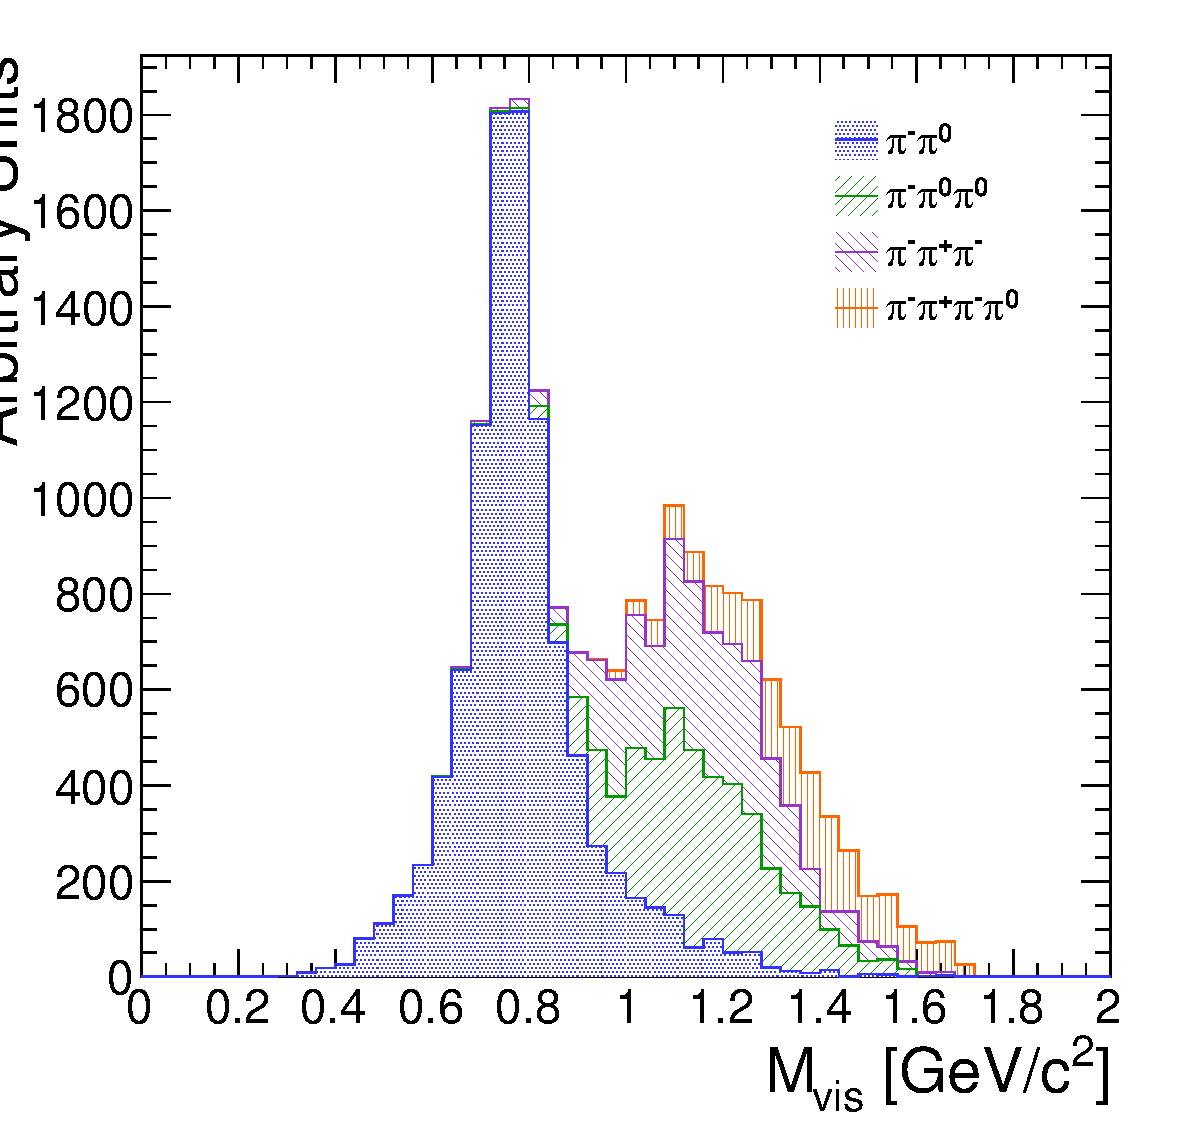
\includegraphics[width=90mm]{tanc_chapter/figures/truthIMvsDM.pdf}
   \end{center}
   \caption[Visible invariant mass of $\tau$ lepton decay products]{The
   invariant mass of the visible decay products in hadronic tau decays.  The
   decay mode $\tau^{-} \to \pi^{-} \nu_\tau$ is omitted.  The different decay
   modes have different invariant masses corresponding to the intermediate
   resonance in the decay.} \label{fig:trueInvMass}
\end{figure}

\section{The Tau Neural Classifier}

The Tau Neural Classifier algorithm reconstructs the decay mode of the
tau--candidate and then feeds the tau--candidate to a discriminator associated
to that decay mode to make the classification decision.  Each discriminator
therefore maps to a reconstructed decay mode in a one-to-one fashion.  To
optimize the discrimination for each of the different decay modes, the TaNC uses
an ensemble of neural nets.  Each neural net corresponds to one of the dominant
hadronic decay modes of the tau lepton.  These selected hadronic decays
constitute 95\% of all hadronic tau decays.  Tau--candidates with reconstructed
decay modes not in the set of dominant hadronic modes are immediately tagged as
background.  

\subsection{Decay mode reconstruction}
\label{sec:decay_mode_reco}
The major task in reconstructing the decay mode of the tau is determining the
number of $\pi^0$ mesons produced in the decay.  A $\pi^0$ meson decays almost
instantaneously to a pair of photons.  The photon objects are reconstructed using the
particle flow algorithm~\cite{CMS-PAS-PFT-09-001}. The initial collection of
photon objects considered to be $\pi^0$ candidates are the photons in the signal
cone described by using the ``shrinking--cone'' tau algorithm, described
elsewhere~\cite{CMS-PAS-PFT-08-001}.  

The reconstruction of photons from $\pi^0$ decays present in the signal cone is
complicated by a number of factors.  To suppress calorimeter noise and underlying
event photons, all photons with minimum transverse energy less than 0.5 GeV are
removed from the signal cone, which removes some signal photons.  Photons
produced in secondary interactions, pile-up events, and electromagnetic showers
produced by signal photons that convert to electron--positron pairs can
contaminate the signal cone with extra low transverse energy photons.  Highly
boosted $\pi^0$ mesons may decay into a pair of photons with a small opening
angle, resulting in two overlapping showers in the ECAL being reconstructed as
one photon.  The $\pi^0$ meson content of the tau candidate is reconstructed in
two stages.  First, photon pairs are merged together into candidate $\pi^0$
mesons.  The remaining unmerged photons are then subjected to a quality
requirement.

\subsubsection{Photon merging}
Photons are merged into composite $\pi^0$ candidates by examining the invariant
mass of all possible pairs of photons in the signal region.  Only $\pi^0$
candidates (photon pairs) with a composite invariant mass less than 0.2 GeV/c
are considered. The combination of the high granularity of the CMS ECAL and the
particle flow algorithm provide excellent energy and angular resolution for
photons; the $\pi^0$ mass peak is readily visible in the invariant mass spectrum
of signal photon pairs (see figure~\ref{fig:imDiPhotonsForTrueDM1}).  The
$\pi^0$ candidates that satisfy the invariant mass requirement are ranked by the
difference between the composite invariant mass of the photon pair and the
invariant mass of the $\pi^0$ meson given by the PDG~\cite{PDG}. The best pairs
are then tagged as $\pi^0$ mesons, removing lower--ranking candidate $\pi^0$s as
necessary to ensure that no photon is included in more than one $\pi^0$ meson.

\begin{figure}[thbp]
  \begin{center}
    \includegraphics*[height=70mm]{tanc_chapter/figures/decayModeMergerAndFilter/invariantMassOfDiPhotonsForDM1.pdf}
    \caption[Invariant mass photon pairs in reconstructed $\pi^0$
    mesons]{Invariant mass of the photon pair for reconstructed
    tau candidates with two reconstructed photons in the signal region
    that are matched to generator level $\tau^{-} \to \pi^{-}\pi^0\nu_\tau$
    decays. }
  \end{center}
  \label{fig:imDiPhotonsForTrueDM1}
\end{figure}


\subsubsection{Quality requirements}
Photons from the underlying event and other reconstruction effects cause the
number of reconstructed photons to be greater than the true number of photons
expected from a given hadronic tau decay.  Photons that have not been merged into
a $\pi^0$ meson candidate are recursively filtered by requiring that the
fraction of the transverse momentum carried by the lowest $P_T$ photon be
greater than 10\% with respect to the entire (tracks, $\pi^0$ candidates, and
photons) tau--candidate. In the case that a photon is not merged but meets the
minimum momentum fraction requirement, it is considered a $\pi^0$
candidate.  This requirement removes extraneous photons, while minimizing the
removal of single photons that correspond to a true $\pi^0$ meson
(see~\ref{fig:photonFiltering}). A mass hypothesis with the
nominal~\cite{PDG} value of the $\pi^0$ is applied to all $\pi^0$ candidates.
All objects that fail the filtering requirements are moved to the isolation
collection.

\begin{figure}[thbp]
  \setlength{\unitlength}{1mm}
  \begin{center}
    \begin{picture}(150, 65)(0,0)
      \put(0.5, 0)
      {\mbox{\includegraphics*[height=60mm]{tanc_chapter/figures/decayModeMergerAndFilter/gammaPtFractionSinglePhotonForDM0.pdf}}}
      % place holder
      \put(78.0, 0)
      {\mbox{\includegraphics*[height=60mm]{tanc_chapter/figures/decayModeMergerAndFilter/gammaPtFractionSinglePhotonForDM1.pdf}}}
    \end{picture}
    \caption[Neutral energy fraction in visible $\tau$ decays]{Fraction of total
    $\tau$-candidate transverse momenta carried by the photon for reconstructed
    taus containing a single photons for two benchmark cases.  On the left, the
    reconstructed tau--candidate is matched to generator level $\tau^{-}
    \rightarrow \pi^{-}\nu_\tau$ decays, for which no photon is expected.  On
    the right, the reconstructed tau--candidate is matched to generator level
    $\tau^{-} \rightarrow \pi^{-}\pi^0\nu_\tau$ decays and the photon is
    expected to correspond to a true $\pi^0$ meson.  The requirement on the
    \pt fraction of the lowest $\pt$ photon improves the purity of the decay
    mode reconstruction.  } \label{fig:photonFiltering}
  \end{center}
\end{figure}


\subsubsection{Performance}
The performance of the decay mode reconstruction can be measured for
tau candidates that are matched to generator level hadronically decaying tau
leptons by examining the correlation of the reconstructed decay mode to the true
decay mode determined from the Monte Carlo generator level information.
Figure~\ref{fig:dmResolution} compares the decay mode reconstruction performance
of a naive approach where the decay mode is determined by simply counting the
number of photons to the performance of the photon merging and filtering
approach described in Section~\ref{sec:decay_mode_reco}.  The correlation for
the merging and filtering algorithm is much more diagonal, indicating higher
performance.  The performance is additonally presented for comparison in tabular form in
Table~\ref{tab:dmResolutionStandard} (merging and filtering approach) and
Table~\ref{tab:dmResolutionNoNothing} (naive approach).

The performance of the decay mode reconstruction is dependent on the transverse
momentum and $\eta$ of the tau candidate and is shown in
Figure~\ref{fig:dmKinematics}.  The \pt dependence is largely due to
threshold effects; high multiplicity decay modes are suppressed at low
transverse momentum as the constituents are below the minimum \pt quality
requirements.  In the forward region, nuclear interactions and conversions from
the increased material budget enhances modes containing $\pi^0$ mesons.


\begin{table}[htp]
   \centering
   \begin{tabular}{l|cccccc}

\multirow{2}{*}{True decay mode} & \multicolumn{6}{c}{Reconstructed Decay Mode}\\

 & $\pi^{-}\nu_\tau$ & $\pi^{-}\pi^0\nu_\tau$ & $\pi^{-}\pi^0\pi^0\nu_\tau$ & $\pi^{-}\pi^{+}\pi^{-}\nu_\tau$ & $\pi^{-}\pi^{+}\pi^{-}\pi^0\nu_\tau$& Other \\
\hline
$\pi^{-}\nu_\tau$ & 14.8\% &1.6\% &0.4\% &0.1\% &0.0\% & 0.7\% \\
$\pi^{-}\pi^0\nu_\tau$ & 6.0\% &17.1\% &9.0\% &0.1\% &0.1\% & 5.5\% \\
$\pi^{-}\pi^0\pi^0\nu_\tau$ & 0.9\% &3.8\% &4.2\% &0.0\% &0.1\% & 5.9\% \\
$\pi^{-}\pi^{+}\pi^{-}\nu_\tau$ & 0.8\% &0.3\% &0.1\% &9.7\% &1.6\% & 6.2\% \\
$\pi^{-}\pi^{+}\pi^{-}\pi^0\nu_\tau$ & 0.1\% &0.2\% &0.1\% &1.7\% &2.7\% & 4.5\% \\

\end{tabular}
\label{tab:dmResolutionNoNothing} \caption[Decay mode performance -- naive
reconstruction]{Decay mode correlation table for the selected dominant decay
modes for the naive approach.  The percentage in a given row and column
indicates the fraction of hadronic tau decays from
$Z\rightarrow\tau^{+}\tau^{-}$ events that are matched to a generator level
decay mode given by the row and are reconstructed with the decay mode given by
the column.  Entries in the "Other" column are immediately tagged as background.
}
\end{table}


\begin{table}[htp]
   \centering
   \begin{tabular}{l|cccccc}

\multirow{2}{*}{True decay mode} & \multicolumn{6}{c}{Reconstructed Decay Mode}\\

 & $\pi^{-}\nu_\tau$ & $\pi^{-}\pi^0\nu_\tau$ & $\pi^{-}\pi^0\pi^0\nu_\tau$ & $\pi^{-}\pi^{+}\pi^{-}\nu_\tau$ & $\pi^{-}\pi^{+}\pi^{-}\pi^0\nu_\tau$& Other \\
\hline
$\pi^{-}\nu_\tau$ & 16.2\% &1.0\% &0.1\% &0.1\% &0.0\% & 0.3\% \\
$\pi^{-}\pi^0\nu_\tau$ & 10.7\% &21.4\% &3.6\% &0.2\% &0.1\% & 1.9\% \\
$\pi^{-}\pi^0\pi^0\nu_\tau$ & 1.8\% &7.1\% &4.4\% &0.1\% &0.0\% & 1.5\% \\
$\pi^{-}\pi^{+}\pi^{-}\nu_\tau$ & 0.9\% &0.2\% &0.0\% &11.5\% &0.6\% & 5.4\% \\
$\pi^{-}\pi^{+}\pi^{-}\pi^0\nu_\tau$ & 0.1\% &0.3\% &0.0\% &3.2\% &2.9\% & 2.7\% \\

\end{tabular}
\label{tab:dmResolutionStandard} \caption[Decay mode performance -- TaNC
reconstruction]{Decay mode correlation table for the selected dominant decay
modes for the merging and filtering approach.  The percentage in a given row and
column indicates the fraction of hadronic tau decays from
$Z\rightarrow\tau^{+}\tau^{-}$ events that are matched to a generator level
decay mode given by the row and are reconstructed with the decay mode given by
the column.  Entries in the "Other" column are immediately tagged as background.
}
\end{table}


\begin{figure}[thbp]
  \centering
   \includegraphics*[width=0.49\textwidth]{tanc_chapter/figures/decayModeMergerAndFilter/dmResolutionStandard.pdf}
   \includegraphics*[width=0.49\textwidth]{tanc_chapter/figures/decayModeMergerAndFilter/dmResolutionNoNothing.pdf}
   \caption[Tau decay mode reconstruction performance]{Correlations between
   reconstructed tau decay mode and true tau decay mode for hadronic tau decays
   in $Z \rightarrow \tau^{+}\tau^{-}$ events.  The correlation when no photon
   merging or filtering is applied is shown on the right, and the correlation
   for the algorithm described in Section~\ref{sec:decay_mode_reco} is on the
   right.  The horizontal and vertical axis are the decay mode indices of the
   true and reconstructed decay mode, respectively.  The decay mode index
   $N_{DM}$ is defined as $N_{DM} = (N_{\pi^{\pm}} - 1)\cdot5 + N_{\pi^0}$.  The
   area of the box in each cell is proportional to the fraction of
   tau candidates that were reconstructed with the decay mode indicated on the
   vertical axis for the true tau decay on the horizontal axis.  The performance
   of a decay mode reconstruction algorithm can be determined by the spread of
   the reconstructed number of $\pi^0$ mesons about the true number (the
   diagonal entries) determined from the generator level Monte Carlo
   information.  If the reconstruction was perfect, the correlation would be
   exactly diagonal.
   %The vertical slice corresponding to each true tau decay mode is normalized;
   %the cells in each column sum to one.
   } \label{fig:dmResolution}
\end{figure}

\begin{figure}[thbp]
   \setlength{\unitlength}{1mm}
   \begin{center}
     \includegraphics*[width=0.99\textwidth]{tanc_chapter/figures/dmVsPt.pdf}
     \includegraphics*[width=0.99\textwidth]{tanc_chapter/figures/dmVsEta.pdf}
   \caption[Kinematic dependence of decay mode reconstruction]{Kinematic
   dependence of reconstructed decay mode for tau candidates in 
   \mbox{$Z\to\tau^{+}\tau^{-}$} (left) and QCD dijets (right) events versus
   transverse momentum (top) and pseudo--rapidity (bottom).  Each curve is the
   probability for a tau candidate to be reconstructed with the associated
   decay mode after the leading pion and decay mode preselection has been
   applied.  } \label{fig:dmKinematics}
   \end{center}
\end{figure}


\subsection{Neural network classification}
\subsubsection{Neural Network Training}
The samples used to train the TaNC neural networks are typical of the signals
and backgrounds found in common physics analyses using taus.  The signal--type
training sample is composed of reconstructed tau candidates that are matched to
generator level hadronic tau decays coming from simulated $\ZTT$ events.  The
background training sample consists of reconstructed tau candidates in
simulated QCD $2\rightarrow2$ hard scattering events.  The QCD $\pt$ spectrum is
steeply falling, and to obtain sufficient statistics across a broad range of
$\pt$ the sample is split into different $\hat \pt$ bins.  Each binned QCD
sample imposes a generator level cut on the transverse momentum of the hard
interaction.  During the evaluation of discrimination performance the QCD
samples are weighted according to their respective integrated luminosities to
remove any effect of the binning.

The signal and background samples are split into five subsamples corresponding
to each reconstructed decay mode.  An additional selection is applied to each
subsample by requiring a ``leading pion'': either a charged hadron or gamma
candidate with transverse momentum greater than 5~\GeVc.  A large number of QCD
training events is required as both the leading pion selection and the
requirement that the decay mode match one of the dominant modes given in
Table~\ref{tab:decay_modes} are effective discriminants.  For each subsample,
80\% of the signal and background tau candidates are used for training the
neural networks, with half (40\%) used as a
validation sample used to ensure the neural network is not over--trained. The
number of signal and background entries used for training and validation in each
decay mode subsample is given in Table~\ref{tab:trainingEvents}.

%Chained 100 signal files.
%Chained 208 background files.
%Total signal entries: 874266
%Total background entries: 9526176
%Pruning non-relevant entries.
%After pruning, 584895 signal and 644315 background entries remain.
%**********************************************************************************
%*********************************** Summary **************************************
%**********************************************************************************
%*     NumEvents with weight > 0 (Total NumEvents)                                *
%*--------------------------------------------------------------------------------*
%*shrinkingConePFTauDecayModeProducer   ThreeProngNoPiZero: Signal:      53257(53271)            Background:155793(155841)
%*shrinkingConePFTauDecayModeProducer  ThreeProngOnePiZero: Signal:      13340(13342)            Background:135871(135942)
%*shrinkingConePFTauDecayModeProducer    OneProngTwoPiZero: Signal:      34780(34799)            Background:51181(51337)
%*shrinkingConePFTauDecayModeProducer    OneProngOnePiZero: Signal:      136464(138171)          Background:137739(139592)
%*shrinkingConePFTauDecayModeProducer     OneProngNoPiZero: Signal:      300951(345312)          Background:144204(161603)

\begin{table}
   \centering
   \begin{tabular}{lcc}
      %\multirow{2}{*}{}                         & \multicolumn{2}{c}{Events}    \\
                                                & Signal        & Background    \\
      \hline
      Total number of tau candidates           & 874266        & 9526176       \\
      Tau candidates passing preselection      & 584895        & 644315        \\
      Tau candidates with $W(\pt,\eta)>0$      & 538792        & 488917        \\
      \hline
      Decay Mode                        & \multicolumn{2}{c}{Training Events}   \\
      \hline
      $\pi^{-}$                         & 300951   & 144204                     \\
      $\pi^{-}\pi^0$                    & 135464   & 137739                     \\
      $\pi^{-}\pi^0\pi^0$               & 34780    & 51181                      \\
      $\pi^{-}\pi^{-}\pi^{+}$           & 53247    & 155793                     \\
      $\pi^{-}\pi^{-}\pi^{+}\pi^0$      & 13340    & 135871                     \\
   \end{tabular}
   \label{tab:trainingEvents} \caption[Neural network training event
   statistics]{Number of events used for neural network training and validation
   for each selected decay mode.}
\end{table}

The remaining 20\% of the signal and background samples are
reserved as a statistically independent sample to evaluate the performance of
the neural nets after the training is completed.  The TaNC uses the Multi--layer
Perceptron (MLP)
neural network implementation provided by the TMVA software package, described
in~\cite{TMVA}.  The MLP classifier is a feed-forward artificial neural
network. There are two layers of hidden nodes and a single node in the output
layer.  The hyperbolic tangent function is used for the neuron activation
function.  

The neural networks used in the TaNC have two hidden layers and single node in
the output layers.  The number of nodes in the first and second hidden layers
are chosen to be $N+1$ and $2N+1$, respectively, where $N$ is the number of
input observables for that neural network.  According to the Kolmogorov's
theorem~\cite{Kolmogorov}, any continuous function $g(x)$ defined on a vector
space of dimension $d$ spanned by $x$ can be represented by
\begin{equation}
   g(x) = \sum_{j=1}^{j=2d+1} \Phi_j \left(\sum_{i=1}^{d} \phi_i(x) \right)
   \label{eq:Kolmogorov}
\end{equation}
for suitably chosen functions for $\Phi_j$ and $\phi_j$.  As the form of
Equation~\ref{eq:Kolmogorov} is similar to the topology of a two hidden--layer
neural network, Kolmogorov's theorem suggests that \emph{any} classification
problem can be solved with a neural network with two hidden layers containing
the appropriate number of nodes.

The neural network is trained for 500 epochs. At ten epoch intervals, the
neural network error is computed using the validation sample to check for
over--training (see Figure~\ref{fig:overTrainCheck}). The neural network error
$E$ is defined~\cite{TMVA} as
\begin{equation}
   E = \frac{1}{2} \sum_{i=1}^N (y_{ANN,i} - \hat y_i)^2
   \label{eq:NNerrorFunc}
   %note - not right for weighted dists?
\end{equation}
where $N$ is the number of training events, $y_{ANN,i}$ is the neural network output
for the $i$th training event, and $y_i$ is the desired (-1 for background, 1 for signal) output
the $i$th event. No evidence  of over--training is observed.

\begin{figure}[thbp]
   \setlength{\unitlength}{1mm}
   \begin{center}
      \begin{picture}(150, 195)(0,0)
         \put(0.5, 130)
         {\mbox{\includegraphics*[height=60mm]{tanc_chapter/figures/overtrainCheck_OneProngNoPiZero.pdf}}}
         \put(65,  130)
         {\mbox{\includegraphics*[height=60mm]{tanc_chapter/figures/overtrainCheck_OneProngOnePiZero.pdf}}}
         \put(0.5, 65) 
         {\mbox{\includegraphics*[height=60mm]{tanc_chapter/figures/overtrainCheck_OneProngTwoPiZero.pdf}}}
         \put(65, 65) 
         {\mbox{\includegraphics*[height=60mm]{tanc_chapter/figures/overtrainCheck_ThreeProngNoPiZero.pdf}}}
         \put(33, 0) 
         {\mbox{\includegraphics*[height=60mm]{tanc_chapter/figures/overtrainCheck_ThreeProngOnePiZero.pdf}}}
      \end{picture}
   \caption[Neural network over--training validation plots]{Neural network
   classification error for training (solid red) and testing (dashed blue)
   samples at ten epoch intervals over the 500 training epochs for each decay
   mode neural network.  The vertical axis represents the classification error,
   defined by equation~\ref{eq:NNerrorFunc}.  N.B. that the choice of hyperbolic
   tangent for neuron activation functions results in the desired outputs for
   signal and background to be 1 and -1, respectively.  This results in the
   computed neural network error being larger by a factor of four than the case
   where the desired outputs are (0, 1).  Classifier over--training would be
   evidenced by divergence of the classification error of the training and
   testing samples, indicating that the neural net was optimizing about
   statistical fluctuations in the training sample.  }
   \label{fig:overTrainCheck}
   \end{center}
\end{figure}


The neural networks use as input observables the transverse momentum and $\eta$
of the tau candidates.  These observables are included as their correlations
with other observables can increase the separation power of the ensemble of
observables.  For example, the opening angle in $\Delta R$ for signal
tau candidates is inversely related to the transverse momentum, while for
background events the correlation is very small~\cite{DavisTau}. In the training
signal and background samples, there is significant discrimination power in the
$\pt$ spectrum.   However, for a general--purpose tau identification algorithm,
it is desirable to eliminate any systematic dependence of the neural network
output on $\pt$ and $\eta$, as in practice the TaNC will be presented with
tau candidates whose $\pt-\eta$ spectrum will be analysis dependent. The
optimal situation would be to train the neural networks using the signal and
backgrounds that are present in the analysis where the algorithm is applied.  In
practice, it is difficult to collect enough training samples for each analysis
situation.  The dependence on $\pt$ and $\eta$ is removed by applying a $\pt$
and $\eta$ dependent weight to the tau candidates when training the neural
nets.  

The weights are defined such that in any region in the vector space spanned by
$\pt$ and $\eta$ where the signal sample and background sample probability
density functions are different, the sample with higher probability density is
weighted such that the samples have identical $\pt-\eta$ probability
distributions.  This removes regions of $\pt-\eta$ space where the training
sample is exclusively signal or background.  The weights are computed according to
\begin{align*}
   W(\pt, \eta) &=  {\rm less}(p_{sig}(\pt, \eta), p_{bkg}(\pt, \eta))\\
   w_{sig}(\pt, \eta) &=  W(\pt, \eta)/p_{sig}(\pt, \eta) \\
   w_{bkg}(\pt, \eta) &=  W(\pt, \eta)/p_{bkg}(\pt, \eta) 
\end{align*}
where \mbox{$p_{sig}(\pt,\eta)$} and \mbox{$p_{bkg}(\pt,\eta)$} are the probability densities of
the signal and background samples after the ``leading pion'' and dominant decay mode
selections. Figure~\ref{fig:nnTrainingWeights} shows the signal and background
training $\pt$ distributions before and after the weighting is applied.


\begin{figure}[thbp]
\setlength{\unitlength}{1mm}
\begin{center}
\includegraphics*[width=0.49\textwidth]{tanc_chapter/figures/training_weights_unweighted.pdf}
\includegraphics*[width=0.49\textwidth]{tanc_chapter/figures/training_weights_weighted.pdf}
%\put(-5.5, 112.5){\small (a)}
%\put(72.0, 112.5){\small (b)}
%\put(-5.5, 54.5){\small (c)}
%\put(72.0, 54.5){\small (d)}
\caption[Kinematic weighting of training sample]{Transverse momentum spectrum of
signal and background tau candidates used in neural net training before (left)
and after (right) the application of \mbox{$\pt-\eta$} dependent weight function.
Application of the weights lowers the training significance of tau candidates
in regions of \mbox{$\pt-\eta$} phase space where either the signal or background
samples has an excess of events. } \label{fig:nnTrainingWeights}
\end{center}
\end{figure} 


\subsubsection{Discriminants}
\label{sec:tanc_nn_discriminants}
Each neural network corresponds to a different decay mode topology and as such
each network uses different observables as inputs.  However, many of the input
observables are used in multiple neural nets.  The superset of all observables
is listed and defined below. Table~\ref{tab:nn_var_table} maps the input
observables to their associated neural networks.  The signal and background
distributions of the input observables for tau--candidates in the training
sample are shown in appendix~\ref{sec:input_descriptions}.  In three prong
decays, the definition of the ``main track'' is important.  The main track
corresponds to the track with charge opposite to that of the total charge of the
three tracks.  This distinction is made to facilitate the use of the ``Dalitz''
observables, allowing identification of intermediate resonances in three--body
decays.  This is motivated by the fact that the three prong decays of the tau
generally proceed through $\tau^{-} \to a1^{-} \nu_\tau \rightarrow
\pi^{-} \rho^0 \nu_\tau \to \pi^{-} \pi^{+} \pi^{-} \nu_\tau$; the
oppositely charged track can always be identified with the $\rho^0$ decay.


\begin{description}
    
  \item[ChargedOutlierAngleN] \hfill \\
  $\Delta R$ between the Nth charged object (ordered by \pt) in the isolation region
    and the tau--candidate momentum axis. If the number of
    isolation region objects is less than N, the input is set at one.

  \item[ChargedOutlierPtN] \hfill \\
  Transverse momentum of the Nth charged object in the isolation region.  If the number of
    isolation region objects is less than N, the input is set at zero.

  \item[DalitzN] \hfill \\
   Invariant mass of four vector sum of the ``main track'' and the Nth signal
    region object. 

  \item[Eta] \hfill \\
  Pseudo-rapidity of the signal region objects. 

  \item[InvariantMassOfSignal] \hfill \\
  Invariant mass of the composite object formed by the signal region constituents.

  \item[MainTrackAngle] \hfill \\
  $\Delta R$ between the ``main track'' and the composite four--vector formed by the 
    signal region constituents.

  \item[MainTrackPt] \hfill \\
  Transverse momentum of the ``main track.'' 

  \item[OutlierNCharged] \hfill \\
  Number of charged objects in the isolation region.

  \item[OutlierSumPt] \hfill \\
  Sum of the transverse momentum of objects in the isolation region.

  \item[PiZeroAngleN] \hfill \\
  $\Delta R$ between the Nth $\pi^0$ object in the signal region (ordered by \pt) and
    the tau--candidate momentum axis.

  \item[PiZeroPtN] \hfill \\
  Transverse momentum of the Nth $\pi^0$ object in the signal region.

  \item[TrackAngleN] \hfill \\
  $\Delta R$ between the Nth charged object in the signal region (ordered by \pt) and
    the tau--candidate momentum axis, exclusive of the main track.

  \item[TrackPtN] \hfill \\
  Transverse momentum of the Nth charged object in the signal region, exclusive of the 
    main track.

\end{description}
    


\begin{table}[h]
   \centering
\begin{tabular}{l|c|c|c|c|c|}
\multirow{2}{*}{Input observable} & \multicolumn{5}{c}{Neural network} \\
 & $\pi^{-}\nu_\tau$ & $\pi^{-}\pi^0\nu_\tau$ & $\pi^{-}\pi^0\pi^0\nu_\tau$ & $\pi^{-}\pi^{+}\pi^{-}\nu_\tau$ & $\pi^{-}\pi^{+}\pi^{-}\pi^0\nu_\tau$\\
\hline
ChargedOutlierAngle1&$\bullet$ & $\bullet$ & $\bullet$ & $\bullet$ & $\bullet$\\
ChargedOutlierAngle2&$\bullet$ & $\bullet$ & $\bullet$ & $\bullet$ & $\bullet$\\
ChargedOutlierPt1&$\bullet$ & $\bullet$ & $\bullet$ & $\bullet$ & $\bullet$\\
ChargedOutlierPt2&$\bullet$ & $\bullet$ & $\bullet$ & $\bullet$ & $\bullet$\\
ChargedOutlierPt3&$\bullet$ & $\bullet$ & $\bullet$ & $\bullet$ & $\bullet$\\
ChargedOutlierPt4&$\bullet$ & $\bullet$ & $\bullet$ & $\bullet$ & $\bullet$\\
Dalitz1& &  & $\bullet$ & $\bullet$ & $\bullet$\\
Dalitz2& &  & $\bullet$ & $\bullet$ & $\bullet$\\
Eta&$\bullet$ & $\bullet$ & $\bullet$ & $\bullet$ & $\bullet$\\
InvariantMassOfSignal& & $\bullet$ & $\bullet$ & $\bullet$ & $\bullet$\\
MainTrackAngle& & $\bullet$ & $\bullet$ & $\bullet$ & $\bullet$\\
MainTrackPt&$\bullet$ & $\bullet$ & $\bullet$ & $\bullet$ & $\bullet$\\
OutlierNCharged&$\bullet$ & $\bullet$ & $\bullet$ & $\bullet$ & $\bullet$\\
OutlierSumPt&$\bullet$ & $\bullet$ & $\bullet$ & $\bullet$ & $\bullet$\\
PiZeroAngle1& & $\bullet$ & $\bullet$ &  & $\bullet$\\
PiZeroAngle2& &  & $\bullet$ &  & \\
PiZeroPt1& & $\bullet$ & $\bullet$ &  & $\bullet$\\
PiZeroPt2& &  & $\bullet$ &  & \\
TrackAngle1& &  &  & $\bullet$ & $\bullet$\\
TrackAngle2& &  &  & $\bullet$ & $\bullet$\\
TrackPt1& &  &  & $\bullet$ & $\bullet$\\
TrackPt2& &  &  & $\bullet$ & $\bullet$\\
\end{tabular}
\caption[Variables used in the different TaNC neural networks]{Input observables
used for each of the neural networks implemented by the Tau Neural Classifier.
The columns represents the neural networks associated to various decay modes and
the rows represent the superset of input observables (see
section~\ref{sec:tanc_nn_discriminants}) used in the neural networks.  A dot in
a given row and column indicates that the observable in that row is used in the
neural network corresponding to that column.  } \label{tab:nn_var_table}

\end{table}


\subsubsection{Neural network performance}
The classification power of the neural networks is unique for each of the decay
modes.  The performance is determined by the relative separation of the signal
and background distributions in the parameter space of the observables used as
neural network inputs.  A pathological example is the case of tau--candidates
with the reconstructed decay mode of $\tau^{-} \to \pi^{-}\nu_\tau$.  If
there is no isolation activity, the neural net has no handle with which it can
separate the signal from the background.  The neural net output for
tau--candidates in the testing sample (independent of the training
and validation samples) for each of the five decay mode classifications is shown
in Figure~\ref{fig:NNoutputDisributions}.

\begin{figure}[thbp]
   \setlength{\unitlength}{1mm}
   \begin{center}
      \begin{picture}(150, 195)(0,0)
         \put(0.5, 130) {\mbox{\includegraphics*[height=60mm]{tanc_chapter/figures/NNOutput_dm_0_pt_20.pdf}}}
         \put(65,  130) {\mbox{\includegraphics*[height=60mm]{tanc_chapter/figures/NNOutput_dm_1_pt_20.pdf}}}
         \put(0.5, 65) {\mbox{\includegraphics*[height=60mm]{tanc_chapter/figures/NNOutput_dm_2_pt_20.pdf}}}
         \put(65, 65) {\mbox{\includegraphics*[height=60mm]{tanc_chapter/figures/NNOutput_dm_10_pt_20.pdf}}}
         \put(33, 0) {\mbox{\includegraphics*[height=60mm]{tanc_chapter/figures/NNOutput_dm_11_pt_20.pdf}}}
      \end{picture}
   \caption[Neural network output in each decay mode]{Neural network output distributions for the
   five reconstructed tau--candidate decay modes used in the TaNC for
   $Z\rightarrow\tau^{+}\tau^{-}$ events (red) and QCD di--jet events (blue).  }
   \label{fig:NNoutputDisributions}
   \end{center}
\end{figure}


When a single neural network is used for classification, choosing an operating
point is relatively straightforward:  the requirement on neural
network output is tuned such that the desired purity is attained.  However, in the case
of the TaNC, multiple neural networks are used.  Each network has a unique
separation power (see Figure~\ref{fig:nnPerfCurves}) and each neural network is
associated to a reconstructed decay mode that composes different relative
fractions of the signal and background tau--candidates.  Therefore, a set of five
numbers is required to define an ``operating point'' (the signal efficiency and
background misidentification rate) in the TaNC output.  All points in this five
dimensional cut--space map to an absolute background fake--rate and signal
efficiency rate.  Therefore there must exist a 5D ``performance curve'' which
for any attainable signal efficiency gives the lowest fake--rate.  A direct
method to approximate the performance curve is possible using a Monte Carlo
technique.   

\begin{figure}[thbp]
   \setlength{\unitlength}{1mm}
   \begin{center}
      \begin{picture}(150, 150)(0,0)
         \put(0.5, 0.5) {\mbox{\includegraphics*[height=150mm]{tanc_chapter/figures/nnPerfCurves_20.pdf}}}
      \end{picture}
   \caption[Performance curves for the neural networks used in the
   TaNC]{Performance curves for the five neural networks used by the TaNC for
   tau--candidates with transverse momentum greater than 20 \GeVc.  Each curve
   represents the signal efficiency (on the horizontal axis) and background
   misidentification rate (vertical axis) for a scan of the neural network
   selection requirement for a single neural network.  The efficiency (or
   misidentification rate) for each neural network performance curve is defined
   with respect to the preselected tau--candidates that have the reconstructed
   decay mode associated with that neural network.  Each neural network has a
   different ability so separate signal and background as each classifier uses
   different observables as inputs.  } \label{fig:nnPerfCurves}
   \end{center}
\end{figure}

The maximal performance curve can be approximated by iteratively sampling points
in the five--dimensional cut space and selecting the highest performance points.
The collection of points in the performance curve are ordered by expected fake
rate.  During each iteration, the sample point is compared to the point before
the potential insertion position of the sample in the ordered collection.  The
sample point is inserted into the collection if it has a higher signal
identification efficiency than the point before it.  The sample point is then
compared to all points in the collection after it (\ie those with a larger fake
rate); any point with a lower signal efficiency than the sample point is
removed.  After the performance curve has been determined, the set of cuts are
evaluated on an independent validation sample to ensure that the measured
performance curve is not influenced by favorable statistical fluctuations being
selected by the Monte Carlo sampling.  The performance curves for two different
transverse momentum ranges are shown in Figure~\ref{fig:mcPerfCurves}.

\begin{figure}[thbp]
   \setlength{\unitlength}{1mm}
   \begin{center}
      \begin{picture}(150, 75)(0,0)
         \put(0.5, 0)
         {\mbox{\includegraphics*[width=75mm]{tanc_chapter/figures/opcurve_test_pt_5.pdf}}}
         \put(15, 60) {$\pt < 20 \GeVc$}
         \put(75, 0)
         {\mbox{\includegraphics*[width=75mm]{tanc_chapter/figures/opcurve_test_pt_20.pdf}}}
         \put(90, 60) {$20 \GeVc <\pt< 50 \GeVc$}
      \end{picture}
   \caption[Tau Neural Classifier performance curves for different \pt
   ranges]{Tau Neural Classifier performance curves for tau--candidates with
   \mbox{$\pt < 20 \GeVc$} (left) and \mbox{$20 <\pt< 50 \GeVc$} (right).  The vertical
   axis represents the expected fake--rate of QCD jets and the horizontal axis
   the expected signal efficiency for hadronic tau decays.  The performance
   curve for the low transverse momentum range is worse due to leading pion
   selection.  While both true taus and QCD are removed by this cut, the
   selection preferentially keeps the QCD tau--candidates with low
   multiplicities, which increases the number of QCD tau--candidates passing the
   decay mode selection.  } \label{fig:mcPerfCurves}
   \end{center}
\end{figure}

The 5D performance curve can also be parameterized by using the probability for
a tau--candidate to be identified for a given decay mode.  
An artificial neural network maps a point in the space of input observables to
some value of neural network output $x$.  The neural network training error is
given by Equation~\ref{eq:NNerrorFunc}.  A given point in the vector space
spanned by the neural network input observables (denoted as ``feature space'')
contributes to the neural network training error $E$ by 
\begin{equation}
   E' = (1 - x)^2\cdot\rho^\tau + x^2\cdot\rho^{QCD}
   \nonumber
\end{equation}
where $\rho^\tau (\rho^{QCD})$ denotes the training sample density of the
$\tau$ signal and QCD--jet background at that point in feature space.

The value $x$ assigned by the neural network to this region in feature space
should satisfy the requirement of minimal error:
\begin{align}
   \frac{\partial E'}{\partial x} &= 0 \nonumber \\ 
   0 &= -2(1-x)\cdot\rho^\tau+2x\cdot\rho^{QCD} \nonumber \\ 
   x &= \frac{\rho^\tau} {\rho^\tau + \rho^{QCD}} \label{eq:probFracToX} \\ 
   \rho^\tau &= x(\rho^\tau + \rho^{QCD}) \nonumber \\ 
   \frac{\rho^{QCD}}{\rho^\tau} &= \frac{1}{x} - 1  \label{eq:rawTransformX}
\end{align}
The ratio $\frac{\rho^{QCD}}{\rho^\tau}$ corresponds to the ratio of
the normalized probability density functions of signal and background input
observable distributions, \ie $\int \rho^{\tau} d\vec x = 1$.

In the case of multiple neural networks, one can derive a formula that maps the
output $x_j$ of the neural network corresponding to decay mode $j$ according to
the ``prior probabilities'' $p_j^\tau (p_j^{QCD})$ for true $\tau$ lepton
hadronic decays (quark and gluon jets) to pass the preselection criteria and
be reconstructed with decay mode $j$.
By substituting $\rho^s \rightarrow \rho^s p_j^s$ for $s \in \{\tau, QCD\}$ in
Equation~\ref{eq:probFracToX}, the output $x_j$ can be related to $p_j^\tau
(p_j^{QCD})$ by 
\begin{equation}
   x_j' = \frac{\rho^\tau \cdot p_j^\tau} 
   {\rho^\tau \cdot p_j^\tau + \rho^{QCD} \cdot p_j^{QCD} }
   = \frac{p_j^\tau} 
   {p_j^\tau + \frac{\rho^{QCD}}{\rho^\tau} \cdot p_j^{QCD} }
   \label{eq:probFracToXWithPriors}
\end{equation}
Substituting Equation~\ref{eq:rawTransformX} into
Equation~\ref{eq:probFracToXWithPriors} yields the transformation of the output
$x_j$ of the neural neural network corresponding to any selected decay mode $j$
to a single discriminator output $x_j'$ which for a given point on the optimal
performance curve should be independent of $j$.
\begin{equation}
   x_j' = \frac{p_j^\tau} 
   {p_j^\tau + \left(\frac{1}{x_j}-1\right)\cdot p_j^{QCD} }
   \label{eq:TransformCut}
\end{equation}
In this manner a single number (the ``transform cut'') given by
Equation~\ref{eq:TransformCut} can be used to specify any point on the
performance curve.  The training sample neural network output after the
transformation has been applied is shown in
Figure~\ref{fig:transformedNNOutput}.  The performance curve for the cut on the
transformed output is nearly identical to the optimal performance curve
determined by the Monte Carlo sampling technique. 

The discriminator output of the TaNC algorithm is a continuous quantity,
enabling analysis specific optimization of the selection to maximize
sensitivity.  For the convenience of the user, four operating point benchmark
selections are provided in addition to the continuous output. The four operating
points are chosen such that for tau--candidates with transverse momentum between
20 and 50~\GeVc, the expected QCD di--jet fake rate will be 0.1\%, 0.25\%,
0.50\% and 1.0\%, respectively.  

\begin{figure}[thbp]
   \setlength{\unitlength}{1mm}
   \begin{center}
      \begin{picture}(150, 75)(0,0)
         \put(0.5, 0)
         {\mbox{\includegraphics*[width=75mm]{tanc_chapter/figures/opcurve_train_pt_20_with_transform.pdf}}}
         \put(14, 60) {20 GeV/c $<\pt<$ 50 GeV/c}
         \put(75, 0)
         {\mbox{\includegraphics*[width=75mm]{tanc_chapter/figures/opcurve_test_pt_20_with_transform.pdf}}}
         \put(90, 60) {20 GeV/c $<\pt<$ 50 GeV/c}
      \end{picture}
   \caption[Tau Neural Classifier transformation performance]{Tau Neural
   Classifier performance curves for tau--candidates with \mbox{$20 < \pt
   < 50 \GeVc$}.  The figure on the left compares the optimal performance curve
   determined by the Monte Carlo sampling method (red) to the performance curve
   obtained by scanning the ``transform cut'' (blue) defined in
   Equation~\ref{eq:TransformCut} from zero to one.  The figure on the right is
   the same set of cuts (and cut transformation values) applied on an
   independent sample to remove any biases introduced by the Monte Carlo
   sampling.  The four dashed lines indicate the performance for the four
   benchmark points.  } \label{fig:tancCurvesWithTransform}
   \end{center}
\end{figure}

\begin{figure}[thbp]
   \setlength{\unitlength}{1mm}
   \begin{center}
      \begin{picture}(75, 75)(0,0)
         \put(0.5, 0.5) {\mbox{\includegraphics*[height=75mm]{tanc_chapter/figures/NNOutput_transform_5_200_preselection.pdf}}}
      \end{picture}
   \caption[Transformed neural network output]{Transformed TaNC neural network
   output for tau--candidates with transverse momentum between 20 and 50~\GeVc
   that pass the pre--selection criteria.  The neural network output for each
   tau--candidate has been transformation according to
   Equation~\ref{eq:TransformCut}.  The decay mode probabilities
   $\rho^{bkg}_i$, $\rho^{signal}_i$ are computed using the entire transverse
   momentum range of the sample.  } \label{fig:transformedNNOutput}
   \end{center}
\end{figure}






\section{Summary}
The Tau Neural classifier introduces two complimentary new techniques for tau
lepton physics at CMS: reconstruction of the hadronic tau decay mode and
discrimination from quark and gluon jets using neural networks.  The decay mode
reconstruction strategy presented in Section~\ref{sec:decay_mode_reco}
significantly improves the determination of the decay mode. This information has
the potential to be useful in studies of tau polarization and background
estimation.

The Tau Neural classifier tau identification algorithm significantly improves
tau discrimination performance compared to isolation--based
approaches~\cite{CMS-PAS-PFT-08-001} used in previous CMS analyses.
Figure~\ref{fig:finalPerfCurve} compares the performance of the ``shrinking
cone'' isolation tau--identification algorithm~\cite{CMS-PAS-PFT-08-001} to the
performance of the TaNC for a scan of requirements on the transformed neural
network output.  The signal efficiency and QCD di--jet fake rate versus
tau--candidate transverse momentum and pseudo--rapidity for the four benchmark
points and the isolation based tau identification are show in
Figure~\ref{fig:kinematicPerformance}.  For tau--candidates with transverse
momentum between 20 and 50~\GeVc, the TaNC operating cut can be chosen such that
the two methods have identical signal efficiency; at this point the TaNC
algorithm reduces the background fake rate by an additional factor of 3.9.  This
reduction in background will directly improve the significance of searches for
new physics using tau leptons at CMS.

\begin{figure}[thbp]
   \setlength{\unitlength}{1mm}
   \begin{center}
      \begin{picture}(150, 150)(0,0)
         \put(0.5, 0.5)
         {\mbox{\includegraphics*[height=150mm]{tanc_chapter/figures/20_pt_50_perf_curve_from_5_pt_200_transform_plain_test_wrt_classic.pdf}}}
      \end{picture}
   \caption[Tau Neural Classifier performance comparison]{Performance curve (red) of the TaNC tau identification for various
   requirements on the output transformed according to
   Equation~\ref{eq:TransformCut}.  The horizontal axis is the efficiency for
   true taus with transverse momentum between 20 and 50~\GeVc to satisfy the tau
   identification requirements.  The vertical axis gives the rate at which QCD
   di--jets with generator--level transverse momentum between 20 and 50 \GeVc
   are incorrectly identified as taus.  The performance point for the same
   tau--candidates using the isolation based tau--identification~\cite{CMS-PAS-PFT-08-001}
   used in many previous CMS analyses is indicated by the black star in the
   figure.  An additional requirement that the signal cone contain one or three
   charged hadrons (typical in a final physics analysis) has been applied to the
   isolation based tau--identification to ensure a conservative comparison.  }
   \label{fig:finalPerfCurve}
   \end{center}
\end{figure}


\begin{figure}[thbp]
   \setlength{\unitlength}{1mm}
   \begin{center}
      \begin{picture}(150, 150)(0,0)
         \put(2.5, 75)
         {\mbox{\includegraphics*[height=70mm]{tanc_chapter/figures/eff_background_pt.pdf}}}
         \put(75,  75)
         {\mbox{\includegraphics*[height=70mm]{tanc_chapter/figures/eff_background_eta.pdf}}}
         \put(2.5, 0)
         {\mbox{\includegraphics*[height=70mm]{tanc_chapter/figures/eff_signal_pt.pdf}}}
         \put(75, 0)
         {\mbox{\includegraphics*[height=70mm]{tanc_chapter/figures/eff_signal_eta.pdf}}}
      \end{picture}
   \caption[Tau Neural Classifier kinematic performance]{Comparison of the
   identification efficiency for hadronic tau decays from $Z \to \tau^{+}
   \tau^{-}$ decays (bottom row) and the misidentification rate for QCD di--jets
   (top row) versus tau--candidate transverse momentum (left) and
   pseudo-rapidity (right) for different tau identification algorithms.  The
   efficiency (fake--rate) in a given bin is defined as the quotient of the
   number of true tau hadronic decays (generator level jets) in that bin that
   are matched to a reconstructed tau--candidate that passes the identification
   algorithm divided by the number of true tau hadronic decays (generator level
   jets) in that bin.  In the low transverse momentum region both the number of
   tau--candidates in the denominator and the algorithm acceptance vary rapidly
   with respect to $\pt$ for both signal and background; a minimum transverse
   momentum requirement of 20 \GeVc is applied to the pseudorapidity plots to
   facilitate interpretation of the plots.  } \label{fig:kinematicPerformance}
   \end{center}
\end{figure}



\section{HPS + TaNC: A Hybrid Algorithm}
\label{sec:TauId} The techniques used in the TaNC have been hybridized with
techniques used by the ``Hadrons plus Strips'' (HPS) algorithm.  The combined
algorithm is referred to ``Hadrons plus Strips and Tau Neural Classifier''
(HPS+TaNC) identification algorithm.  The algorithm combines features of
HPS~\cite{CMS_AN_2010-082} and the TaNC algorithm.  Both algorithms are based on
reconstructing individual tau lepton hadronic decay modes, which has been
demonstrated to improve the tau identification performance significantly with
respect to previously used cone isolation based
algorithms~\cite{CMS-PAS-PFT-10-004}.  The HPS+TaNC algorithm first reconstructs
the hadronic decay mode of the tau, and applies different discriminants based on
the reconstructed decay mode.  Identification of hadronic tau decays by the
HPS+TaNC algorithm proceeds in two stages: first, the hadronic decay mode of the
tau is reconstructed and then different discriminators are applied, based on the
reconstructed decay mode.  In the decay mode reconstruction particular attention
is paid to the reconstruction of neutral pions, which are expected for the
majority of hadronic decay modes.


\subsubsection{Decay mode reconstruction}

The decay mode reconstruction algorithm is seeded by particle--flow jets
reconstructed by the anti--$k_{T}$ algorithm~\cite{AntiKT}.  In order to
reconstruct the decay mode, the algorithm needs to merge photon candidates into
candidate $\pi^0$ mesons.  $\pi^0$ candidates are reconstructed by two
algorithms which are executed concurrently.  The ``combinatoric'' $\pi^0$
algorithm produces a $\pi^0$ candidate for every possible pair of photons within
the jet.  The ``strips'' algorithm clusters photons strips in $\eta-\phi$.  The
results of both algorithms are combined and then ``cleaned'', resolving multiple
hypotheses.  The quality of a $\pi^0$ candidate is determined according to the
following categorical rankings:
\begin{itemize}
\item The $\pi^0$ candidate is in the ECAL barrel region ($|\eta| < 1.5$) 
and has invariant mass $|m_{\gamma \gamma} - m_{\pi^0}| < 0.05~\GeVcc$.
\item The $\pi^0$ candidate is in the ECAL endcap region ($|\eta| > 1.5$)
 and has invariant mass $m_{\gamma \gamma} < 0.2~\GeVcc$.
\item The $\pi^0$ candidate contains two or more photons within an $\eta-\phi$ strip of size $0.05 \times 0.20$.
\item Photons not satisfying any of the other categories are considered as
  unresolved $\pi^0$ candidates in case they have $\pt > 1.0~\GeVc$.
\end{itemize}  
$m_{\pi^0}$ denotes the nominal neutral pion mass~\cite{PDG}.  The choice of the
invariant mass windows in the ECAL endcap and barrel regions is motivated by the
resolution on the $\pi^0$ mass (illustrated in Figure~\ref{fig:PFPiZeroRes})
measured in particle--flow commissioning~\cite{CMS-PAS-PFT-10-002}.  Multiple
$\pi^0$ candidates in the same category are ranked in quality according to the
difference of the reconstructed photon pair mass to the nominal $\pi^0$ mass.
After the $\pi^0$ candidates are ranked, the highest ranked candidate is
selected for the final collection.  The photon constituents of the highest
ranked candidate are removed from remaining $\pi^0$ candidates not yet selected
for the final collection in order to prevent photons from entering more than one
$\pi^0$ candidate.  The rank of remaining $\pi^0$ candidates is reevaluated and
the $\pi^0$ candidate with the next highest rank is selected for the output
collection.  The process is repeated until no more $\pi^0$ candidates are
remaining.
\begin{figure}[thbp]
  \centering
  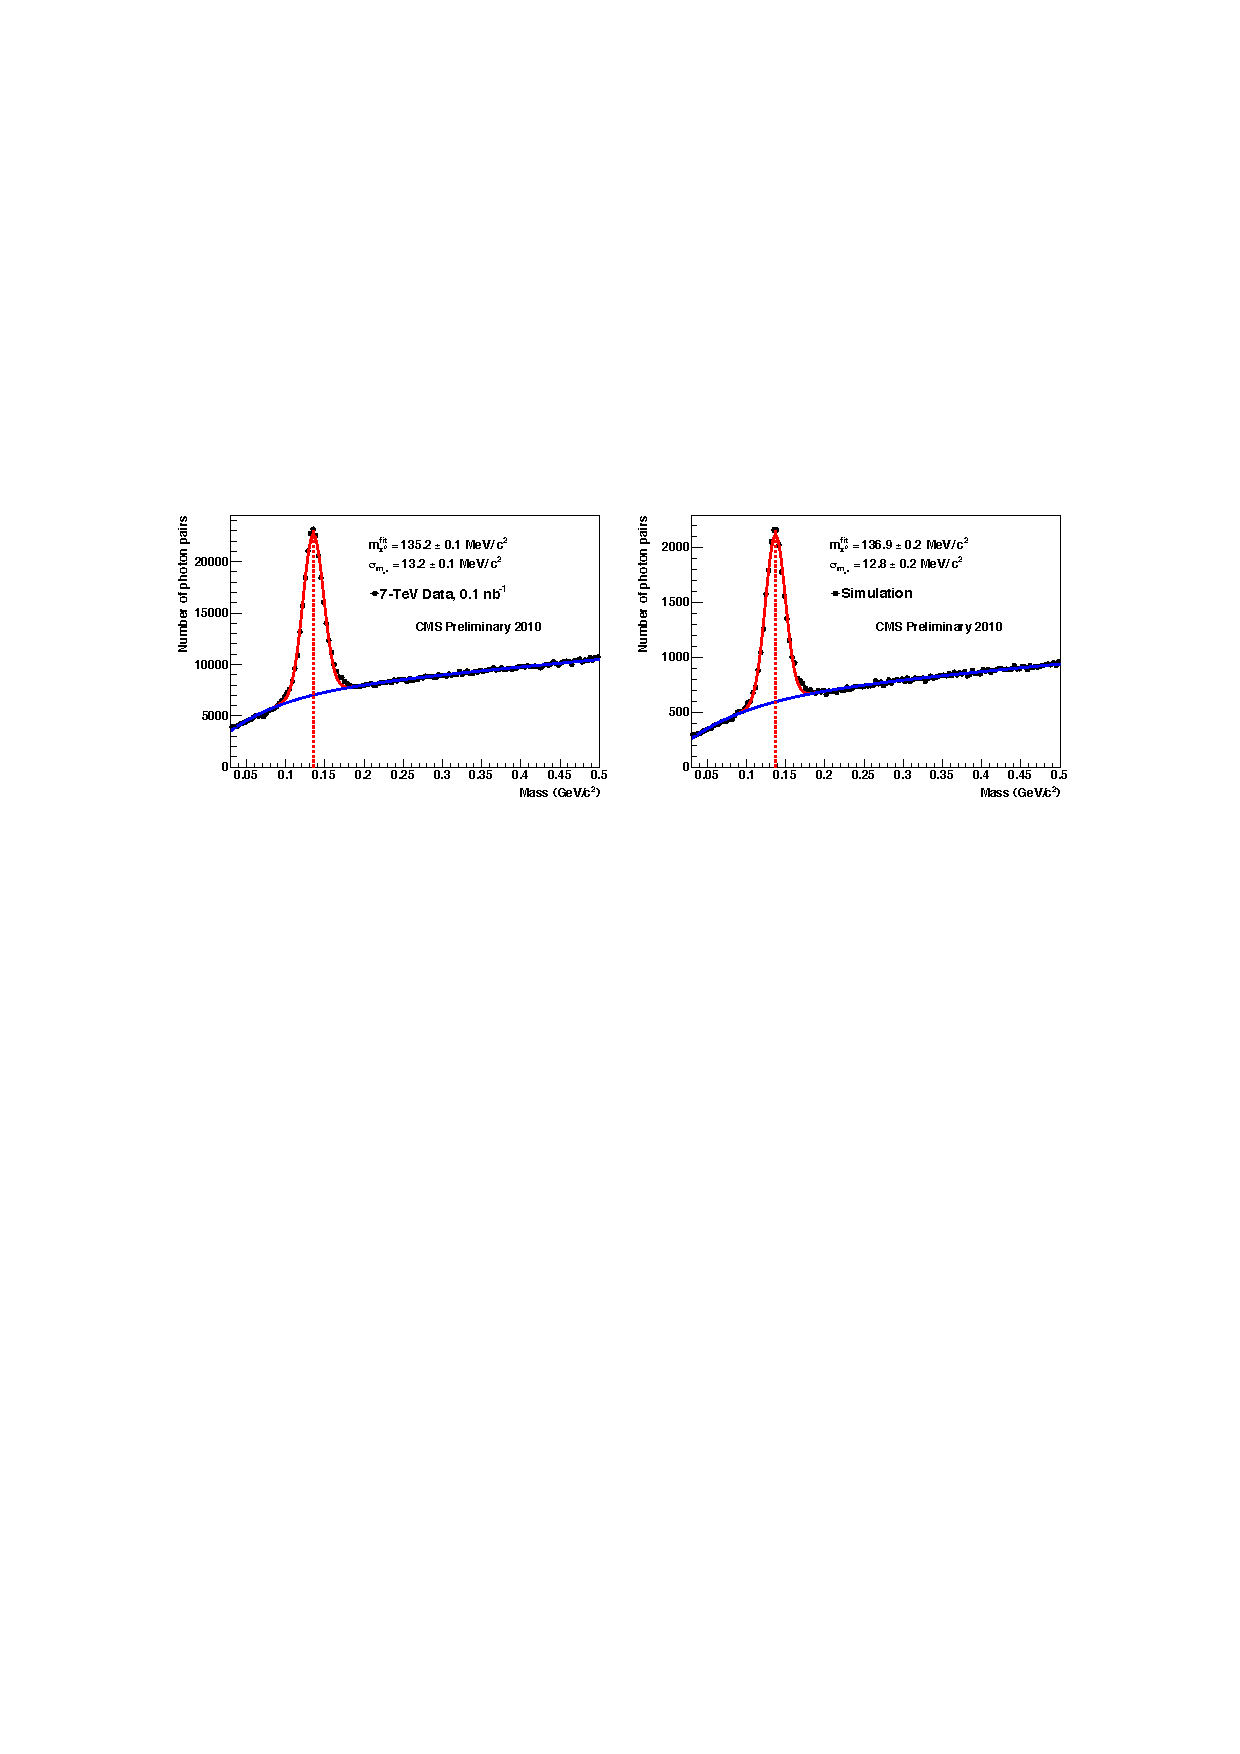
\includegraphics[width=0.95\textwidth]{tanc_chapter/figures/PFPiZeroRes.pdf}
  \caption[Invariant mass distribution of PF photon pairs]{Invariant mass
  distribution of photon pairs reconstructed by the particle--flow in 2010 CMS
  minimum bias events (left), and predicted by the simulation (right).  A clear
  resonant pick corresponding to the $\pi_0$ meson is visible above the
  combinatoric background. Reference:~\cite{CMS-PAS-PFT-10-002}}
  \label{fig:PFPiZeroRes}
\end{figure}

Once the final collection of $\pi^0$ candidates is determined, tau
reconstruction in the HPS+TaNC algorithm proceeds by building tau candidates
from reconstructed $\pi^0$ candidates and charged hadrons reconstructed by the
particle--flow algorithm.  A combinatoric approach is again employed for the tau
candidate building.  A tau candidate hypothesis is built for every combination
of jet constituents ($\pi^0$ candidates plus charged hadrons) which has a
multiplicity consistent with a hadronic tau decay.  The tau candidates are
ranked analogous to the ranking utilized for the $\pi^0$ reconstruction, but
with the following categorical rankings:
\begin{itemize}
\item In each decay mode category, the tau candidate with the highest neural network output is selected.
\item The tau candidate has unit charge.
\item The tau candidate passes the ``lead pion'' criteria, requiring that there
  is a photon or charged pion candidate with $\pt > 5~\GeVc$.
\item The tau candidate passes the HPS invariant mass and 
  collimation\footnote{The invariant mass of the signal candidates is required
  to be compatible with the resolution for that decay mode.  The collimation
  selection requires the maximum $\Delta R$ between any two signal candidates to
  be less than $2.8/\et$, where \et is the total transverse energy of the signal
  candidates.  A full description is available in~\cite{CMS_AN_2010-082}.}
  requirements.
\end{itemize}  
In case multiple tau candidates satisfy all four categorical requirements,  the
tau candidate with the highest energy sum of charged and neutral pions is
selected as the highest ranking one.

\subsubsection{Hadronic tau discrimination}

The final level of discrimination is performed by an ensemble of neural
networks, with each neural network corresponding to a specific decay mode,
analogously to the method used original TaNC algorithm
(Section~\ref{sec:tanc_nn_training}).  The inputs of
each neural network are different and correspond to the observables (invariant
mass, Dalitz masses) available for its associated decay mode.  The neural
networks are trained on samples simulated $Z \to \TT$ events
(``signal'') and QCD di--jet events selected in the 7~\TeV data collected by CMS
in 2010 (``background'').  All of the tau hypothesis from a given jet
reconstructed in data are used for training.  The $Z \to \tau^+\tau^-$
signal sample is generated by PYTHIA~\cite{pythia6_4} which has been interfaced
TAUOLA~\cite{tauola} for the purpose of generating the tau decays and simulated
passed through the ``full'' GEANT~\cite{geant} based simulation of the CMS
detector.  Only tau candidates which have been reconstructed in a decay mode
matching the true decay mode of the tau on generator level enter the signal
training sample.  The neural network implementation, network layout, and
training strategies are the same as in the original TaNC algorithm described in
this chapter.  To account
for differences in the input signal purity and separation power of the neural
networks between decay modes, the outputs of each neural network are transformed
according to the method described in~\cite{CMS_AN_2010-099}.  Multiple
working--points, corresponding to different purities are provided. 

\ifx\master\undefined% AUTOCOMPILE
% Allows for individual chapters to be compiled.

% Usage:
% \ifx\master\undefined% AUTOCOMPILE
% Allows for individual chapters to be compiled.

% Usage:
% \ifx\master\undefined% AUTOCOMPILE
% Allows for individual chapters to be compiled.

% Usage:
% \ifx\master\undefined\input{../settings/autocompile}\fi
% (place at start and end of chapter file)

\ifx\noprelim\undefined
    % first time included
    % input preamble files
    \input{../settings/phdsetup}

    \begin{document}
    \def\noprelim{}
\else
    % already included once
    % input post files

    \singlespacing
    \bibliographystyle{../bibliography/expanded}
    \bibliography{../bibliography/references}

    \end{document}
\fi\fi
% (place at start and end of chapter file)

\ifx\noprelim\undefined
    % first time included
    % input preamble files
    % [ USER VARIABLES ]

\def\PHDTITLE {Extensions of the Theory of Computational Mechanics}
\def\PHDAUTHOR{Evan Klose Friis}
\def\PHDSCHOOL{University of California, Davis}

\def\PHDMONTH {June}
\def\PHDYEAR  {2011}
\def\PHDDEPT {Physics}

\def\BSSCHOOL {University of California at San Diego}
\def\BSYEAR   {2005}

\def\PHDCOMMITTEEA{Professor John Conway}
\def\PHDCOMMITTEEB{Professor Robin Erbacher}
\def\PHDCOMMITTEEC{Professor Mani Tripathi}

% [ GLOBAL SETUP ]

\documentclass[letterpaper,oneside,11pt]{report}

\usepackage{calc}
\usepackage{breakcites}
\usepackage[newcommands]{ragged2e}

\usepackage[pdftex]{graphicx}
\usepackage{epstopdf}

%\usepackage{tikz}
%\usetikzlibrary{positioning} % [right=of ...]
%\usetikzlibrary{fit} % [fit= ...]

%\pgfdeclarelayer{background layer}
%\pgfdeclarelayer{foreground layer}
%\pgfsetlayers{background layer,main,foreground layer}

%\newenvironment{wrap}{\noindent\begin{minipage}[t]{\linewidth}\vspace{-0.5\normalbaselineskip}\centering}{\vspace{0.5\normalbaselineskip}\end{minipage}}

%% [Venn diagram environment]
%\newenvironment{venn2}
%{\begin{tikzpicture} [every pin/.style={text=black, text opacity=1.0, pin distance=0.5cm, pin edge={black!60, semithick}},
%% define a new style 'venn'
%venn/.style={circle, draw=black!60, semithick, minimum size = 4cm}]
%
%% create circle and give it external (pin) label
%\node[venn] (X) at (-1,0) [pin={150:$H[X]$}] {};
%\node[venn] (Y) at (1,0) [pin={30:$H[Y]$}] {};
%
%% place labels of the atoms by hand
%\node at (-1.9,0) {$H[X|Y]$};
%\node at (1.9,0) {$H[Y|X]$};
%\node at (0,0) {$I[X;Y]$};}
%{\end{tikzpicture}}

%\newcommand{\wrapmath}[1]{\begin{wrap}\begin{tikzpicture}[every node/.style={inner ysep=0ex, inner xsep=0em}]\node[] {$\displaystyle\begin{aligned} #1\end{aligned}$};\end{tikzpicture}\end{wrap}}

\renewenvironment{abstract}{\chapter*{Abstract}}{}
\renewcommand{\bibname}{Bibliography}
\renewcommand{\contentsname}{Table of Contents}

\makeatletter
\renewcommand{\@biblabel}[1]{\textsc{#1}}
\makeatother

% [ FONT SETTINGS ]

\usepackage[tbtags, intlimits, namelimits]{amsmath}
\usepackage[adobe-utopia]{mathdesign}

\DeclareSymbolFont{pazomath}{OMS}{zplm}{m}{n}
\DeclareSymbolFontAlphabet{\mathcal}{pazomath}
\SetMathAlphabet\mathcal{bold}{OMS}{zplm}{b}{n}

\SetSymbolFont{largesymbols}{normal}{OMX}{zplm}{m}{n}
\SetSymbolFont{largesymbols}{bold}{OMX}{zplm}{m}{n}
\SetSymbolFont{symbols}{normal}{OMS}{zplm}{m}{n}
\SetSymbolFont{symbols}{bold}{OMS}{zplm}{b}{n}

\renewcommand{\sfdefault}{phv}
\renewcommand{\ttdefault}{fvm}

\widowpenalty 8000
\clubpenalty  8000

% [ PAGE LAYOUT ]
\usepackage{geometry}
\geometry{lmargin = 1.5in}
\geometry{rmargin = 1.0in}
\geometry{tmargin = 1.0in}
\geometry{bmargin = 1.0in}

% [ PDF SETTINGS ]

\usepackage[final]{hyperref}
\hypersetup{breaklinks  = true}
\hypersetup{colorlinks  = true}
\hypersetup{linktocpage = false}
\hypersetup{linkcolor   = blue}
\hypersetup{citecolor   = green}
\hypersetup{urlcolor    = black}
\hypersetup{plainpages  = false}
\hypersetup{pageanchor  = true}
\hypersetup{pdfauthor   = {\PHDAUTHOR}}
\hypersetup{pdftitle    = {\PHDTITLE}}
\hypersetup{pdfsubject  = {Dissertation, \PHDSCHOOL}}
\urlstyle{same}

% [ LETTER SPACING ]

\usepackage[final]{microtype}
\microtypesetup{protrusion=compatibility}
\microtypesetup{expansion=false}

\newcommand{\upper}[1]{\MakeUppercase{#1}}
\let\lsscshape\scshape

\ifcase\pdfoutput\else\microtypesetup{letterspace=15}
\renewcommand{\scshape}{\lsscshape\lsstyle}
\renewcommand{\upper}[1]{\textls[50]{\MakeUppercase{#1}}}\fi

% [ LINE SPACING ]

\usepackage[doublespacing]{setspace}
\renewcommand{\displayskipstretch}{0.0}

\setlength{\parskip   }{0em}
\setlength{\parindent }{2em}

% [ TABLE FORMATTING ]

\usepackage{booktabs}
\setlength{\heavyrulewidth}{1.5\arrayrulewidth}
\setlength{\lightrulewidth}{1.0\arrayrulewidth}
\setlength{\doublerulesep }{2.0\arrayrulewidth}

% [ SECTION FORMATTING ]

\usepackage[largestsep,nobottomtitles*]{titlesec}
\renewcommand{\bottomtitlespace}{0.75in}

\titleformat{\chapter}[display]{\bfseries\huge\singlespacing}{\filleft\textsc{\LARGE \chaptertitlename\ \thechapter}}{-0.2ex}{\titlerule[3pt]\vspace{0.2ex}}[]

\titleformat{\section}{\LARGE}{\S\thesection\hspace{0.5em}}{0ex}{}
\titleformat{\subsection}{\Large}{\S\thesubsection\hspace{0.5em}}{0ex}{}
\titleformat{\subsubsection}{\large}{\thesubsubsection\hspace{0.5em}}{0ex}{}

\titlespacing*{\chapter}{0em}{6ex}{4ex plus 2ex minus 0ex}
\titlespacing*{\section}{0em}{2ex plus 3ex minus 1ex}{0.5ex plus 0.5ex minus 0.5ex}
\titlespacing*{\subsection}{0ex}{2ex plus 3ex minus 1ex}{0ex}
\titlespacing*{\subsubsection}{0ex}{2ex plus 0ex minus 1ex}{0ex}

% [ HEADER SETTINGS ]

\usepackage{fancyhdr}

\setlength{\headheight}{\normalbaselineskip}
\setlength{\footskip  }{0.5in}
\setlength{\headsep   }{0.5in-\headheight}

\fancyheadoffset[R]{0.5in}
\renewcommand{\headrulewidth}{0pt}
\renewcommand{\footrulewidth}{0pt}

\newcommand{\pagebox}{\parbox[r][\headheight][t]{0.5in}{\hspace\fill\thepage}}

\newcommand{\prelimheaders}{\ifx\prelim\undefined\renewcommand{\thepage}{\textit{\roman{page}}}\fancypagestyle{plain}{\fancyhf{}\fancyfoot[L]{\makebox[\textwidth-0.5in]{\thepage}}}\pagestyle{plain}\def\prelim{}\fi}

\newcommand{\normalheaders}{\renewcommand{\thepage}{\arabic{page}}\fancypagestyle{plain}{\fancyhf{}\fancyhead[R]{\pagebox}}\pagestyle{plain}}

\normalheaders{}

% [ CUSTOM COMMANDS ]

\newcommand{\signaturebox}[1]{\multicolumn{1}{p{4in}}{\vspace{3ex}}\\\midrule #1\\}

%\input{../includes/cmechabbrev}

% [some math stuff - maybe stick in sep file]
\usepackage{amsthm}
\usepackage{amscd}
\theoremstyle{plain}    \newtheorem{Lem}{Lemma}
\theoremstyle{plain}    \newtheorem*{ProLem}{Proof}
\theoremstyle{plain} 	\newtheorem{Cor}{Corollary}
\theoremstyle{plain} 	\newtheorem*{ProCor}{Proof}
\theoremstyle{plain} 	\newtheorem{The}{Theorem}
\theoremstyle{plain} 	\newtheorem*{ProThe}{Proof}
\theoremstyle{plain} 	\newtheorem{Prop}{Proposition}
\theoremstyle{plain} 	\newtheorem*{ProProp}{Proof}
\theoremstyle{plain} 	\newtheorem*{Conj}{Conjecture}
\theoremstyle{plain}	\newtheorem*{Rem}{Remark}
\theoremstyle{plain}	\newtheorem*{Def}{Definition} 
\theoremstyle{plain}	\newtheorem*{Not}{Notation}

% [uniform figure scaling - maybe this is not a good idea]
\def\figscale{.7}
\def\lscale{1.0}

% [FIX ME! - red makes it easier to spot]
\newcommand{\FIX}[1]{\textbf{\textcolor{red}{#1}}}


    \begin{document}
    \def\noprelim{}
\else
    % already included once
    % input post files

    \singlespacing
    \bibliographystyle{../bibliography/expanded}
    \bibliography{../bibliography/references}

    \end{document}
\fi\fi
% (place at start and end of chapter file)

\ifx\noprelim\undefined
    % first time included
    % input preamble files
    % [ USER VARIABLES ]

\def\PHDTITLE {Extensions of the Theory of Computational Mechanics}
\def\PHDAUTHOR{Evan Klose Friis}
\def\PHDSCHOOL{University of California, Davis}

\def\PHDMONTH {June}
\def\PHDYEAR  {2011}
\def\PHDDEPT {Physics}

\def\BSSCHOOL {University of California at San Diego}
\def\BSYEAR   {2005}

\def\PHDCOMMITTEEA{Professor John Conway}
\def\PHDCOMMITTEEB{Professor Robin Erbacher}
\def\PHDCOMMITTEEC{Professor Mani Tripathi}

% [ GLOBAL SETUP ]

\documentclass[letterpaper,oneside,11pt]{report}

\usepackage{calc}
\usepackage{breakcites}
\usepackage[newcommands]{ragged2e}

\usepackage[pdftex]{graphicx}
\usepackage{epstopdf}

%\usepackage{tikz}
%\usetikzlibrary{positioning} % [right=of ...]
%\usetikzlibrary{fit} % [fit= ...]

%\pgfdeclarelayer{background layer}
%\pgfdeclarelayer{foreground layer}
%\pgfsetlayers{background layer,main,foreground layer}

%\newenvironment{wrap}{\noindent\begin{minipage}[t]{\linewidth}\vspace{-0.5\normalbaselineskip}\centering}{\vspace{0.5\normalbaselineskip}\end{minipage}}

%% [Venn diagram environment]
%\newenvironment{venn2}
%{\begin{tikzpicture} [every pin/.style={text=black, text opacity=1.0, pin distance=0.5cm, pin edge={black!60, semithick}},
%% define a new style 'venn'
%venn/.style={circle, draw=black!60, semithick, minimum size = 4cm}]
%
%% create circle and give it external (pin) label
%\node[venn] (X) at (-1,0) [pin={150:$H[X]$}] {};
%\node[venn] (Y) at (1,0) [pin={30:$H[Y]$}] {};
%
%% place labels of the atoms by hand
%\node at (-1.9,0) {$H[X|Y]$};
%\node at (1.9,0) {$H[Y|X]$};
%\node at (0,0) {$I[X;Y]$};}
%{\end{tikzpicture}}

%\newcommand{\wrapmath}[1]{\begin{wrap}\begin{tikzpicture}[every node/.style={inner ysep=0ex, inner xsep=0em}]\node[] {$\displaystyle\begin{aligned} #1\end{aligned}$};\end{tikzpicture}\end{wrap}}

\renewenvironment{abstract}{\chapter*{Abstract}}{}
\renewcommand{\bibname}{Bibliography}
\renewcommand{\contentsname}{Table of Contents}

\makeatletter
\renewcommand{\@biblabel}[1]{\textsc{#1}}
\makeatother

% [ FONT SETTINGS ]

\usepackage[tbtags, intlimits, namelimits]{amsmath}
\usepackage[adobe-utopia]{mathdesign}

\DeclareSymbolFont{pazomath}{OMS}{zplm}{m}{n}
\DeclareSymbolFontAlphabet{\mathcal}{pazomath}
\SetMathAlphabet\mathcal{bold}{OMS}{zplm}{b}{n}

\SetSymbolFont{largesymbols}{normal}{OMX}{zplm}{m}{n}
\SetSymbolFont{largesymbols}{bold}{OMX}{zplm}{m}{n}
\SetSymbolFont{symbols}{normal}{OMS}{zplm}{m}{n}
\SetSymbolFont{symbols}{bold}{OMS}{zplm}{b}{n}

\renewcommand{\sfdefault}{phv}
\renewcommand{\ttdefault}{fvm}

\widowpenalty 8000
\clubpenalty  8000

% [ PAGE LAYOUT ]
\usepackage{geometry}
\geometry{lmargin = 1.5in}
\geometry{rmargin = 1.0in}
\geometry{tmargin = 1.0in}
\geometry{bmargin = 1.0in}

% [ PDF SETTINGS ]

\usepackage[final]{hyperref}
\hypersetup{breaklinks  = true}
\hypersetup{colorlinks  = true}
\hypersetup{linktocpage = false}
\hypersetup{linkcolor   = blue}
\hypersetup{citecolor   = green}
\hypersetup{urlcolor    = black}
\hypersetup{plainpages  = false}
\hypersetup{pageanchor  = true}
\hypersetup{pdfauthor   = {\PHDAUTHOR}}
\hypersetup{pdftitle    = {\PHDTITLE}}
\hypersetup{pdfsubject  = {Dissertation, \PHDSCHOOL}}
\urlstyle{same}

% [ LETTER SPACING ]

\usepackage[final]{microtype}
\microtypesetup{protrusion=compatibility}
\microtypesetup{expansion=false}

\newcommand{\upper}[1]{\MakeUppercase{#1}}
\let\lsscshape\scshape

\ifcase\pdfoutput\else\microtypesetup{letterspace=15}
\renewcommand{\scshape}{\lsscshape\lsstyle}
\renewcommand{\upper}[1]{\textls[50]{\MakeUppercase{#1}}}\fi

% [ LINE SPACING ]

\usepackage[doublespacing]{setspace}
\renewcommand{\displayskipstretch}{0.0}

\setlength{\parskip   }{0em}
\setlength{\parindent }{2em}

% [ TABLE FORMATTING ]

\usepackage{booktabs}
\setlength{\heavyrulewidth}{1.5\arrayrulewidth}
\setlength{\lightrulewidth}{1.0\arrayrulewidth}
\setlength{\doublerulesep }{2.0\arrayrulewidth}

% [ SECTION FORMATTING ]

\usepackage[largestsep,nobottomtitles*]{titlesec}
\renewcommand{\bottomtitlespace}{0.75in}

\titleformat{\chapter}[display]{\bfseries\huge\singlespacing}{\filleft\textsc{\LARGE \chaptertitlename\ \thechapter}}{-0.2ex}{\titlerule[3pt]\vspace{0.2ex}}[]

\titleformat{\section}{\LARGE}{\S\thesection\hspace{0.5em}}{0ex}{}
\titleformat{\subsection}{\Large}{\S\thesubsection\hspace{0.5em}}{0ex}{}
\titleformat{\subsubsection}{\large}{\thesubsubsection\hspace{0.5em}}{0ex}{}

\titlespacing*{\chapter}{0em}{6ex}{4ex plus 2ex minus 0ex}
\titlespacing*{\section}{0em}{2ex plus 3ex minus 1ex}{0.5ex plus 0.5ex minus 0.5ex}
\titlespacing*{\subsection}{0ex}{2ex plus 3ex minus 1ex}{0ex}
\titlespacing*{\subsubsection}{0ex}{2ex plus 0ex minus 1ex}{0ex}

% [ HEADER SETTINGS ]

\usepackage{fancyhdr}

\setlength{\headheight}{\normalbaselineskip}
\setlength{\footskip  }{0.5in}
\setlength{\headsep   }{0.5in-\headheight}

\fancyheadoffset[R]{0.5in}
\renewcommand{\headrulewidth}{0pt}
\renewcommand{\footrulewidth}{0pt}

\newcommand{\pagebox}{\parbox[r][\headheight][t]{0.5in}{\hspace\fill\thepage}}

\newcommand{\prelimheaders}{\ifx\prelim\undefined\renewcommand{\thepage}{\textit{\roman{page}}}\fancypagestyle{plain}{\fancyhf{}\fancyfoot[L]{\makebox[\textwidth-0.5in]{\thepage}}}\pagestyle{plain}\def\prelim{}\fi}

\newcommand{\normalheaders}{\renewcommand{\thepage}{\arabic{page}}\fancypagestyle{plain}{\fancyhf{}\fancyhead[R]{\pagebox}}\pagestyle{plain}}

\normalheaders{}

% [ CUSTOM COMMANDS ]

\newcommand{\signaturebox}[1]{\multicolumn{1}{p{4in}}{\vspace{3ex}}\\\midrule #1\\}

%%%% macros fro standard references
%\eqref provided by amsmath
\newcommand{\figref}[1]{Fig.~\ref{#1}}
\newcommand{\tableref}[1]{Table~\ref{#1}}
\newcommand{\refcite}[1]{Ref.~\cite{#1}}

% Abbreviations from CMPPSS:

\newcommand{\eM}     {\mbox{$\epsilon$-machine}}
\newcommand{\eMs}    {\mbox{$\epsilon$-machines}}
\newcommand{\EM}     {\mbox{$\epsilon$-Machine}}
\newcommand{\EMs}    {\mbox{$\epsilon$-Machines}}
\newcommand{\eT}     {\mbox{$\epsilon$-transducer}}
\newcommand{\eTs}    {\mbox{$\epsilon$-transducers}}
\newcommand{\ET}     {\mbox{$\epsilon$-Transducer}}
\newcommand{\ETs}    {\mbox{$\epsilon$-Transducers}}

% Processes and sequences

\newcommand{\Process}{\mathcal{P}}

\newcommand{\ProbMach}{\Prob_{\mathrm{M}}}
\newcommand{\Lmax}   { {L_{\mathrm{max}}}}
\newcommand{\MeasAlphabet}	{\mathcal{A}}
% Original
%\newcommand{\MeasSymbol}   { {S} }
%\newcommand{\meassymbol}   { {s} }
% New symbol
\newcommand{\MeasSymbol}   { {X} }
\newcommand{\meassymbol}   { {x} }
\newcommand{\BiInfinity}	{ \overleftrightarrow {\MeasSymbol} }
\newcommand{\biinfinity}	{ \overleftrightarrow {\meassymbol} }
\newcommand{\Past}	{ \overleftarrow {\MeasSymbol} }
\newcommand{\past}	{ {\overleftarrow {\meassymbol}} }
\newcommand{\pastprime}	{ {\past}^{\prime}}
\newcommand{\Future}	{ \overrightarrow{\MeasSymbol} }
\newcommand{\future}	{ \overrightarrow{\meassymbol} }
\newcommand{\futureprime}	{ {\future}^{\prime}}
\newcommand{\PastPrime}	{ {\Past}^{\prime}}
\newcommand{\FuturePrime}	{ {\overrightarrow{\meassymbol}}^\prime }
\newcommand{\PastDblPrime}	{ {\overleftarrow{\meassymbol}}^{\prime\prime} }
\newcommand{\FutureDblPrime}	{ {\overrightarrow{\meassymbol}}^{\prime\prime} }
\newcommand{\pastL}	{ {\overleftarrow {\meassymbol}}{}^L }
\newcommand{\PastL}	{ {\overleftarrow {\MeasSymbol}}{}^L }
\newcommand{\PastLt}	{ {\overleftarrow {\MeasSymbol}}_t^L }
\newcommand{\PastLLessOne}	{ {\overleftarrow {\MeasSymbol}}^{L-1} }
\newcommand{\futureL}	{ {\overrightarrow{\meassymbol}}{}^L }
\newcommand{\FutureL}	{ {\overrightarrow{\MeasSymbol}}{}^L }
\newcommand{\FutureLt}	{ {\overrightarrow{\MeasSymbol}}_t^L }
\newcommand{\FutureLLessOne}	{ {\overrightarrow{\MeasSymbol}}^{L-1} }
\newcommand{\pastLprime}	{ {\overleftarrow {\meassymbol}}^{L^\prime} }
\newcommand{\futureLprime}	{ {\overrightarrow{\meassymbol}}^{L^\prime} }
\newcommand{\AllPasts}	{ { \overleftarrow {\rm {\bf \MeasSymbol}} } }
\newcommand{\AllFutures}	{ \overrightarrow {\rm {\bf \MeasSymbol}} }
\newcommand{\FutureSet}	{ \overrightarrow{\bf \MeasSymbol}}

% Causal states and epsilon-machines
\newcommand{\CausalState}	{ \mathcal{S} }
\newcommand{\CausalStatePrime}	{ {\CausalState}^{\prime}}
\newcommand{\causalstate}	{ \sigma }
\newcommand{\CausalStateSet}	{ \boldsymbol{\CausalState} }
\newcommand{\AlternateState}	{ \mathcal{R} }
\newcommand{\AlternateStatePrime}	{ {\cal R}^{\prime} }
\newcommand{\alternatestate}	{ \rho }
\newcommand{\alternatestateprime}	{ {\rho^{\prime}} }
\newcommand{\AlternateStateSet}	{ \boldsymbol{\AlternateState} }
\newcommand{\PrescientState}	{ \widehat{\AlternateState} }
\newcommand{\prescientstate}	{ \widehat{\alternatestate} }
\newcommand{\PrescientStateSet}	{ \boldsymbol{\PrescientState}}
\newcommand{\CausalEquivalence}	{ {\sim}_{\epsilon} }
\newcommand{\CausalEquivalenceNot}	{ {\not \sim}_{\epsilon}}

\newcommand{\NonCausalEquivalence}	{ {\sim}_{\eta} }
\newcommand{\NextObservable}	{ {\overrightarrow {\MeasSymbol}}^1 }
\newcommand{\LastObservable}	{ {\overleftarrow {\MeasSymbol}}^1 }
%\newcommand{\Prob}		{ {\rm P}}
\newcommand{\Prob}      {\Pr} % use standard command
\newcommand{\ProbAnd}	{ {,\;} }
\newcommand{\LLimit}	{ {L \rightarrow \infty}}
\newcommand{\Cmu}		{C_\mu}
\newcommand{\hmu}		{h_\mu}
\newcommand{\EE}		{{\bf E}}
\newcommand{\Measurable}{{\bf \mu}}

% Process Crypticity
\newcommand{\PC}		{\chi}
\newcommand{\FuturePC}		{\PC^+}
\newcommand{\PastPC}		{\PC^-}
% Causal Irreversibility
\newcommand{\CI}		{\Xi}
\newcommand{\ReverseMap}	{r}
\newcommand{\ForwardMap}	{f}

% Abbreviations from IB:
% None that aren't already in CMPPSS

% Abbreviations from Extensive Estimation:
\newcommand{\EstCausalState}	{\widehat{\CausalState}}
\newcommand{\estcausalstate}	{\widehat{\causalstate}}
\newcommand{\EstCausalStateSet}	{\boldsymbol{\EstCausalState}}
\newcommand{\EstCausalFunc}	{\widehat{\epsilon}}
\newcommand{\EstCmu}		{\widehat{\Cmu}}
\newcommand{\PastLOne}	{{\Past}^{L+1}}
\newcommand{\pastLOne}	{{\past}^{L+1}}

% Abbreviations from $\epsilon$-Transducers:
\newcommand{\InAlphabet}	{ \mathcal{A}}
\newcommand{\insymbol}		{ a}
\newcommand{\OutAlphabet}	{ \mathcal{B}}
\newcommand{\outsymbol}		{ b}
\newcommand{\InputSimple}	{ X}
\newcommand{\inputsimple}	{ x}
\newcommand{\BottleneckVar}	{\tilde{\InputSimple}}
\newcommand{\bottleneckvar}	{\tilde{\inputsimple}}
\newcommand{\InputSpace}	{ \mathbf{\InputSimple}}
\newcommand{\InputBi}	{ \overleftrightarrow {\InputSimple} }
\newcommand{\inputbi}	{ \overleftrightarrow {\inputsimple} }
\newcommand{\InputPast}	{ \overleftarrow {\InputSimple} }
\newcommand{\inputpast}	{ \overleftarrow {\inputsimple} }
\newcommand{\InputFuture}	{ \overrightarrow {\InputSimple} }
\newcommand{\inputfuture}	{ \overrightarrow {\inputsimple} }
\newcommand{\NextInput}	{ {{\InputFuture}^{1}}}
\newcommand{\NextOutput}	{ {\OutputFuture}^{1}}
\newcommand{\OutputSimple}	{ Y}
\newcommand{\outputsimple}	{ y}
\newcommand{\OutputSpace}	{ \mathbf{\OutputSimple}}
\newcommand{\OutputBi}	{ \overleftrightarrow{\OutputSimple} }
\newcommand{\outputbi}	{ \overleftrightarrow{\outputsimple} }
\newcommand{\OutputPast}	{ \overleftarrow{\OutputSimple} }
\newcommand{\outputpast}	{ \overleftarrow{\outputsimple} }
\newcommand{\OutputFuture}	{ \overrightarrow{\OutputSimple} }
\newcommand{\outputfuture}	{ \overrightarrow{\outputsimple} }
\newcommand{\OutputL}	{ {\OutputFuture}^L}
\newcommand{\outputL}	{ {\outputfuture}^L}
\newcommand{\InputLLessOne}	{ {\InputFuture}^{L-1}}
\newcommand{\inputLlessone}	{ {\inputufutre}^{L-1}}
\newcommand{\OutputPastLLessOne}	{{\OutputPast}^{L-1}_{-1}}
\newcommand{\outputpastLlessone}	{{\outputpast}^{L-1}}
\newcommand{\OutputPastLessOne}	{{\OutputPast}_{-1}}
\newcommand{\outputpastlessone}	{{\outputpast}_{-1}}
\newcommand{\OutputPastL}	{{\OutputPast}^{L}}
\newcommand{\OutputLPlusOne}	{ {\OutputFuture}^{L+1}}
\newcommand{\outputLplusone}	{ {\outputfutre}^{L+1}}
\newcommand{\InputPastL}	{{\InputPast}^{L}}
\newcommand{\inputpastL}	{{\inputpast}^{L}}
\newcommand{\JointPast}	{{(\InputPast,\OutputPast)}}
\newcommand{\jointpast}	{{(\inputpast,\outputpast)}}
\newcommand{\jointpastone}	{{(\inputpast_1,\outputpast_1)}}
\newcommand{\jointpasttwo}	{{(\inputpast_2,\outputpast_2)}}
\newcommand{\jointpastprime} {{({\inputpast}^{\prime},{\outputpast}^{\prime})}}
\newcommand{\NextJoint}	{{(\NextInput,\NextOutput)}}
\newcommand{\nextjoint}	{{(\insymbol,\outsymbol)}}
\newcommand{\AllInputPasts}	{ { \overleftarrow {\rm \InputSpace}}}
\newcommand{\AllOutputPasts}	{ {\overleftarrow {\rm \OutputSpace}}}
\newcommand{\DetCausalState}	{ {{\cal S}_D }}
\newcommand{\detcausalstate}	{ {{\sigma}_D} }
\newcommand{\DetCausalStateSet}	{ \boldsymbol{{\CausalState}_D}}
\newcommand{\DetCausalEquivalence}	{ {\sim}_{{\epsilon}_{D}}}
\newcommand{\PrescientEquivalence}	{ {\sim}_{\widehat{\eta}}}
\newcommand{\FeedbackCausalState}	{ \mathcal{F}}
\newcommand{\feedbackcausalstate}	{ \phi}
\newcommand{\FeedbackCausalStateSet}	{ \mathbf{\FeedbackCausalState}}
\newcommand{\JointCausalState}		{ \mathcal{J}}
\newcommand{\JointCausalStateSet}	{ \mathbf{\JointCausalState}}
\newcommand{\UtilityFunctional}	{ {\mathcal{L}}}
\newcommand{\NatureState}	{ {\Omega}}
\newcommand{\naturestate}	{ {\omega}}
\newcommand{\NatureStateSpace}	{ {\mathbf{\NatureState}}}
\newcommand{\AnAction}	{ {A}}
\newcommand{\anaction}	{ {a}}
\newcommand{\ActionSpace}	{ {\mathbf{\AnAction}}}

% Abbreviations from RURO:
\newcommand{\InfoGain}[2] { \mathcal{D} \left( {#1} || {#2} \right) }

% Abbreviations from Upper Bound:
\newcommand{\lcm}	{{\rm lcm}}
% Double-check that this isn't in the math set already!

% Abbreviations from Emergence in Space
\newcommand{\ProcessAlphabet}	{\MeasAlphabet}
\newcommand{\ProbEst}			{ {\widehat{\Prob}_N}}
\newcommand{\STRegion}			{ {\mathrm K}}
\newcommand{\STRegionVariable}		{ K}
\newcommand{\stregionvariable}		{ k}
\newcommand{\GlobalPast}		{ \overleftarrow{G}} 
\newcommand{\globalpast}		{ \overleftarrow{g}} 
\newcommand{\GlobalFuture}		{ \overrightarrow{G}}
\newcommand{\globalfuture}		{ \overrightarrow{g}}
\newcommand{\GlobalState}		{ \mathcal{G}}
\newcommand{\globalstate}		{ \gamma}
\newcommand{\GlobalStateSet}		{ {\mathbf \GlobalState}}
\newcommand{\LocalPast}			{ \overleftarrow{L}} 
\newcommand{\localpast}			{ \overleftarrow{l}}
\newcommand{\AllLocalPasts}		{ \mathbf{\LocalPast}}
\newcommand{\LocalPastRegion}		{ \overleftarrow{\mathrm L}}
\newcommand{\LocalFuture}		{ \overrightarrow{L}}
\newcommand{\localfuture}		{ \overrightarrow{l}}
\newcommand{\LocalFutureRegion}		{ \overrightarrow{\mathrm L}}
\newcommand{\LocalState}		{ \mathcal{L}}
\newcommand{\localstate}		{ \lambda}
\newcommand{\LocalStateSet}		{ {\mathbf \LocalState}}
\newcommand{\PatchPast}			{ \overleftarrow{P}}
\newcommand{\patchpast}			{ \overleftarrow{p}}
\newcommand{\PatchPastRegion}		{ \overleftarrow{\mathrm P}}
\newcommand{\PatchFuture}		{ \overrightarrow{P}}
\newcommand{\patchfuture}		{ \overrightarrow{p}}
\newcommand{\PatchFutureRegion}		{ \overrightarrow{\mathrm P}}
\newcommand{\PatchState}		{ \mathcal{P}}
\newcommand{\patchstate}		{ \pi}
\newcommand{\PatchStateSet}		{ {\mathbf \PatchState}}
\newcommand{\LocalStatesInPatch}	{\vec{\LocalState}}
\newcommand{\localstatesinpatch}	{\vec{\localstate}}
\newcommand{\PointInstantX}		{ {\mathbf x}}
% Galles's original LaTeX for the cond. indep. symbol follows:
\newcommand{\compos}{\mbox{$~\underline{~\parallel~}~$}}
\newcommand{\ncompos}{\not\hspace{-.15in}\compos}
\newcommand{\indep}			{ \rotatebox{90}{$\models$}}
\newcommand{\nindep}	{\not\hspace{-.05in}\indep}
\newcommand{\LocalEE}	{{\EE}^{loc}}
\newcommand{\EEDensity}	{\overline{\LocalEE}}
\newcommand{\LocalCmu}	{{\Cmu}^{loc}}
\newcommand{\CmuDensity}	{\overline{\LocalCmu}}

%%%%%%%%%%% added by sasa
\newcommand{\FinPast}[1]	{ \overleftarrow {\MeasSymbol} \stackrel{{#1}}{}}
\newcommand{\finpast}[1]  	{ \overleftarrow {\meassymbol}  \stackrel{{#1}}{}}
\newcommand{\FinFuture}[1]		{ \overrightarrow{\MeasSymbol} \stackrel{{#1}}{}}
\newcommand{\finfuture}[1]		{ \overrightarrow{\meassymbol} \stackrel{{#1}}{}}

\newcommand{\Partition}	{ \AlternateState }
\newcommand{\partitionstate}	{ \alternatestate }
\newcommand{\PartitionSet}	{ \AlternateStateSet }
\newcommand{\Fdet}   { F_{\rm det} }

\newcommand{\Dkl}[2] { D_{\rm KL} \left( {#1} || {#2} \right) }

\newcommand{\Period}	{p}

% To take into account time direction
\newcommand{\forward}{+}
\newcommand{\reverse}{-}
%\newcommand{\forwardreverse}{\:\!\diamond} % \pm
\newcommand{\forwardreverse}{\pm} % \pm
\newcommand{\FutureProcess}	{ {\Process}^{\forward} }
\newcommand{\PastProcess}	{ {\Process}^{\reverse} }
\newcommand{\FutureCausalState}	{ {\CausalState}^{\forward} }
\newcommand{\futurecausalstate}	{ \sigma^{\forward} }
\newcommand{\altfuturecausalstate}	{ \sigma^{\forward\prime} }
\newcommand{\PastCausalState}	{ {\CausalState}^{\reverse} }
\newcommand{\pastcausalstate}	{ \sigma^{\reverse} }
\newcommand{\BiCausalState}		{ {\CausalState}^{\forwardreverse} }
\newcommand{\bicausalstate}		{ {\sigma}^{\forwardreverse} }
\newcommand{\FutureCausalStateSet}	{ {\CausalStateSet}^{\forward} }
\newcommand{\PastCausalStateSet}	{ {\CausalStateSet}^{\reverse} }
\newcommand{\BiCausalStateSet}	{ {\CausalStateSet}^{\forwardreverse} }
\newcommand{\eMachine}	{ M }
\newcommand{\FutureEM}	{ {\eMachine}^{\forward} }
\newcommand{\PastEM}	{ {\eMachine}^{\reverse} }
\newcommand{\BiEM}		{ {\eMachine}^{\forwardreverse} }
\newcommand{\BiEquiv}	{ {\sim}^{\forwardreverse} }
\newcommand{\Futurehmu}	{ h_\mu^{\forward} }
\newcommand{\Pasthmu}	{ h_\mu^{\reverse} }
\newcommand{\FutureCmu}	{ C_\mu^{\forward} }
\newcommand{\PastCmu}	{ C_\mu^{\reverse} }
\newcommand{\BiCmu}		{ C_\mu^{\forwardreverse} }
\newcommand{\FutureEps}	{ \epsilon^{\forward} }
\newcommand{\PastEps}	{ \epsilon^{\reverse} }
\newcommand{\BiEps}	{ \epsilon^{\forwardreverse} }
\newcommand{\FutureSim}	{ \sim^{\forward} }
\newcommand{\PastSim}	{ \sim^{\reverse} }
% Used arrows for awhile, more or less confusing?
%\newcommand{\FutureCausalState}	{ \overrightarrow{\CausalState} }
%\newcommand{\PastCausalState}	{ \overleftarrow{\CausalState} }
%\newcommand{\eMachine}	{ M }
%\newcommand{\FutureEM}	{ \overrightarrow{\eMachine} }
%\newcommand{\PastEM}	{ \overleftarrow{\eMachine} }
%\newcommand{\FutureCmu}	{ \overrightarrow{\Cmu} }
%\newcommand{\PastCmu}	{ \overleftarrow{\Cmu} }

%% time-reversing and mixed state presentation operators
\newcommand{\TR}{\mathcal{T}}
\newcommand{\MSP}{\mathcal{U}}
\newcommand{\one}{\mathbf{1}}

%% (cje)
%% Provide a command \ifpm which is true when \pm 
%% is meant to be understood as "+ or -". This is
%% different from the usage in TBA.
\newif\ifpm 
\edef\tempa{\forwardreverse}
\edef\tempb{\pm}
\ifx\tempa\tempb
   \pmfalse
\else
   \pmtrue  
\fi





% [some math stuff - maybe stick in sep file]
\usepackage{amsthm}
\usepackage{amscd}
\theoremstyle{plain}    \newtheorem{Lem}{Lemma}
\theoremstyle{plain}    \newtheorem*{ProLem}{Proof}
\theoremstyle{plain} 	\newtheorem{Cor}{Corollary}
\theoremstyle{plain} 	\newtheorem*{ProCor}{Proof}
\theoremstyle{plain} 	\newtheorem{The}{Theorem}
\theoremstyle{plain} 	\newtheorem*{ProThe}{Proof}
\theoremstyle{plain} 	\newtheorem{Prop}{Proposition}
\theoremstyle{plain} 	\newtheorem*{ProProp}{Proof}
\theoremstyle{plain} 	\newtheorem*{Conj}{Conjecture}
\theoremstyle{plain}	\newtheorem*{Rem}{Remark}
\theoremstyle{plain}	\newtheorem*{Def}{Definition} 
\theoremstyle{plain}	\newtheorem*{Not}{Notation}

% [uniform figure scaling - maybe this is not a good idea]
\def\figscale{.7}
\def\lscale{1.0}

% [FIX ME! - red makes it easier to spot]
\newcommand{\FIX}[1]{\textbf{\textcolor{red}{#1}}}


    \begin{document}
    \def\noprelim{}
\else
    % already included once
    % input post files

    \singlespacing
    \bibliographystyle{../bibliography/expanded}
    \bibliography{../bibliography/references}

    \end{document}
\fi\fi
